%%
%% getstart.tex -- Flight Gear documentation: The FlightGear Manual
%% Chapter file
%%
%% Copyright (C) 2002 Michael Basler
%%                  & Bernhard Buckel
%%
%% This program is free software; you can redistribute it and/or
%% modify it under the terms of the GNU General Public License as
%% published by the Free Software Foundation; either version 2 of the
%% License, or (at your option) any later version.
%%
%% This program is distributed in the hope that it will be useful, but
%% WITHOUT ANY WARRANTY; without even the implied warranty of
%% MERCHANTABILITY or FITNESS FOR A PARTICULAR PURPOSE.  See the GNU
%% General Public License for more details.
%%
%% You should have received a copy of the GNU General Public License
%% along with this program; if not, write to the Free Software
%% Foundation, Inc., 675 Mass Ave, Cambridge, MA 02139, USA.
%%
%% $Id: takeof.tex,v 0.6 2002/09/09 michael
%% (Log is kept at end of this file)

%%%%%%%%%%%%%%%%%%%%%%%%%%%%%%%%%%%%%%%%%%%%%%%%%%%%%%%%%%%%%%%%%%%%%%%%%%%%%%%%%%%%%%%%%%%%%%%
\iflanguage{english}{
\chapter{Takeoff: How to start the program}
}{}
\iflanguage{french}{
\chapter{D\'{e}collage : comment d\'{e}marrer le programme}
}{}
\label{takeoff}
%%%%%%%%%%%%%%%%%%%%%%%%%%%%%%%%%%%%%%%%%%%%%%%%%%%%%%%%%%%%%%%%%%%%%%%%%%%%%%%%%%%%%%%%%%%%%%%
\markboth{\thechapter.\hspace*{1mm}
TAKEOFF}{\thesection\hspace*{1mm} Command line parameters}


%%%%%%%%%%%%%%%%%%%%%%%%%%%%%%%%%%%%%%%%%%%%%%%%%%%%%%%%%%%%%%%%%%%%%%%%%%%%%%%%%%%%%%%%%%%%%%%
\iflanguage{english}{
\section{Environment Variables}\index{environment variables}
}{}
\iflanguage{french}{
\section{Variables d'environnement}\index{variables d'environment}
}{}
%%%%%%%%%%%%%%%%%%%%%%%%%%%%%%%%%%%%%%%%%%%%%%%%%%%%%%%%%%%%%%%%%%%%%%%%%%%%%%%%%%%%%%%%%%%%%%%

\iflanguage{english}{
There are two environment variables that must be defined to run \FlightGear{}.
These tell \FlightGear{} where to find its data and scenery.

You can set them in a number of ways depending on your platform and requirements. 
}{}
\iflanguage{french}{
Il existe deux variables d'environnement qui doivent \^{e}tre d\'{e}finies pour faire fonctionner \FlightGear{}.
Elles indiquent \`{a} \FlightGear{} o\`{u} trouver ses donn\'{e}es et ses sc\`{e}nes.

Vous pouvez les param\'{e}trer de plusieurs fa\c{c}ons en fonction de votre plate-forme et de vos besoins.
}{}

\subsection{FG\_ROOT}\index{FG\_ROOT}

\iflanguage{english}{
This is where \FlightGear{} will find data files such as aircraft, navigational
beacon locations, airport frequencies. This is the \texttt{data} subdirectory
of where you installed \FlightGear{}. e.g.
\texttt{/usr/local/share/FlightGear/data} or
\texttt{c:$\backslash$Program Files$\backslash$FlightGear$\backslash$data}.
}{}
\iflanguage{french}{
Il s'agit de l'emplacement o\`{u} \FlightGear{} recherchera ses fichiers de donn\'{e}es comme
les a\'{e}ronefs, les emplacements des balises de navigation, les fr\'{e}quences des a\'{e}roports. Il s'agit du
sous-r\'{e}pertoire \texttt{data} de l'emplacement o\`{u} vous avez install\'{e} \FlightGear{}, par exemple :
\texttt{/usr/local/share/FlightGear/data} ou
\texttt{c:$\backslash$Program Files$\backslash$FlightGear$\backslash$data}.
}{}

\subsection{FG\_SCENERY}\index{FG\_SCENERY}

\iflanguage{english}{
This is where \FlightGear{} will look for scenery files. It consists of a list
of directories that will be searched in order. The directories are separated
by ``:'' on Unix and ``;'' on Windows. e.g.
}{}
\iflanguage{french}{
Il s'agit de l'emplacement o\`{u} \FlightGear{} recherchera ses fichiers de sc\`{e}nes. Il s'agit
d'une liste de r\'{e}pertoires qui seront analys\'{e}s de mani\`{e}re s\'{e}quentielle. Les r\'{e}pertoires
sont s\'{e}par\'{e}s par ``:'' sous Unix et ``;'' sous Windows, par exemple :
}{}

\noindent
{\footnotesize{\texttt{/home/joebloggs/WorldScenery:/usr/local/share/FlightGear/data/Scenery}}}

\noindent
\iflanguage{english}{
or
}{}
\iflanguage{french}{
ou
}{}

\noindent
{\footnotesize{\texttt{c:$\backslash$Program Files$\backslash$FlightGear$\backslash$data$\backslash$Scenery;c:$\backslash$Program Files$\backslash$FlightGear$\backslash$data$\backslash$WorldScenery}}}.

\iflanguage{english}{
\subsection{Environment Variables on Windows and Mac OS X}
The graphical wizard on Windows and the GUI launcher on Mac OS X internally
define these environment variables so you don't have to define these yourself.
However, in case you launch \FlightGear{} from command-line, you need to
explicitly define these variables.
}{}
\iflanguage{french}{
\subsection{Variables d'environnement sous Windows et Mac OS X}
Les assistants graphiques sous Windows et le GUI launcher sous Mac OS X d\'{e}finissent
de mani\`{e}re interne ces variables d'environnement de telle sorte que vous n'avez pas besoin de les d\'{e}finir vous-m\^{e}me.
Cependant, si jamais vous lancez \FlightGear{} depuis la ligne de commande, vous devez d\'{e}finir ces variables de mani\`{e}re
explicite.
}{}

%%%%%%%%%%%%%%%%%%%%%%%%%%%%%%%%%%%%%%%%%%%%%%%%%%%%%%%%%%%%%%%%%%%%%%%%%%%%%%%%%%%%%%%%%%%%%%%
\iflanguage{english}{
\section{Launching the simulator under Unix/Linux}\index{Launching Flightgear!Linux}\index{Starting Flightgear!Linux}
}{}
\iflanguage{french}{
\section{D\'{e}marrer le simulateur sous Unix/Linux}\index{D\'{e}marrer Flightgear!Linux}\index{D\'{e}marrer Flightgear!Linux}
}{}
%%%%%%%%%%%%%%%%%%%%%%%%%%%%%%%%%%%%%%%%%%%%%%%%%%%%%%%%%%%%%%%%%%%%%%%%%%%%%%%%%%%%%%%%%%%%%%%

\centerline{\fbox{
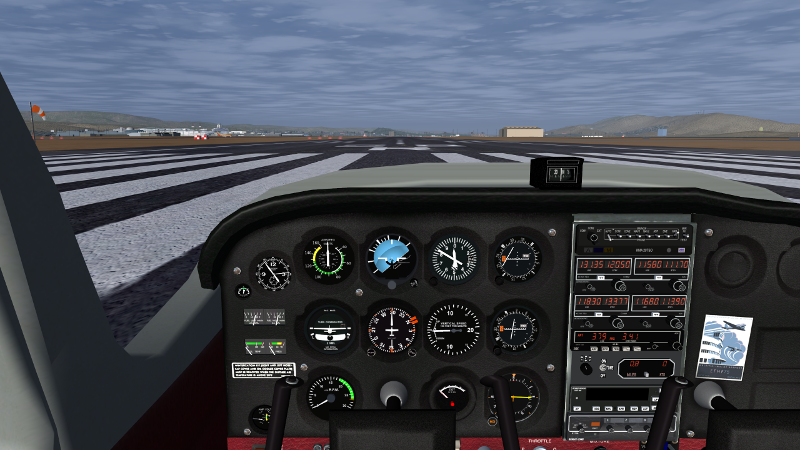
\includegraphics[clip,width=12.5cm]{img/ksfo}
}}
\smallskip
 \noindent

\iflanguage{english}{
Fig.\,3: Ready for takeoff: \textit{Waiting at the default startup position at San
Francisco Intl., KSFO.}
}{}
\iflanguage{french}{
Fig.\,3 : Par\'{e} \`{a} d\'{e}coller : \textit{en attente \`{a} la position de d\'{e}marrage par d\'{e}faut de l'a\'{e}roport de San
Francisco Intl., KSFO.}
}{}
\medskip

\iflanguage{english}{
Before you can run \FlightGear{}, you need to set a couple of environment variables:
}{}
\iflanguage{french}{
Avant de pouvoir d\'{e}marrer \FlightGear{}, vous devez d\'{e}finir deux variables d'environnement :
}{}

\begin{itemize}
\iflanguage{english}{
\item You must add \texttt{/usr/local/share/FlightGear/lib} to your \texttt{LD\_LIBRARY\_PATH}
\item \texttt{FG\_ROOT} must be set to the data directory of your \FlightGear{} installation. e.g. \texttt{/usr/local/share/FlightGear/data}.
\item \texttt{FG\_SCENERY} should be a list of scenery directories, separated by '':''. This works like \texttt{PATH} when searching for scenery.
e.g. \texttt{\$FG\_ROOT/Scenery:\$FG\_ROOT/WorldScenery}.
}{}

\iflanguage{french}{
\item Vous devez ajouter \texttt{/usr/local/share/FlightGear/lib} \`{a} votre \texttt{LD\_LIBRARY\_PATH}
\item \texttt{FG\_ROOT} doit \^{e}tre param\'{e}tr\'{e} pour pointer vers le r\'{e}pertoire contenant les donn\'{e}es de votre installation de  \FlightGear{}, par exemple : \texttt{/usr/local/share/FlightGear/data}.
\item \texttt{FG\_SCENERY} doit \^{e}tre une liste de r\'{e}pertoires de sc\`{e}nes, s\'{e}par\'{e}s par '':''. Ce fonctionnement est semblable \`{a} celui de \texttt{PATH} lorsqu'on recherche des sc\`{e}nes.
par exemple : \texttt{\$FG\_ROOT/Scenery:\$FG\_ROOT/WorldScenery}.
}{}

\end{itemize}

\noindent
\iflanguage{english}{
To add these in the Bourne shell (and compatibles):
}{}
\iflanguage{french}{
Pour les ajouter dans le Bourne shell (et compatibles) :
}{}
\begin{verbatim}
LD_LIBRARY_PATH=/usr/local/share/FlightGear/lib:$LD_LIBRARY_PATH
export LD_LIBRARY_PATH
FG_HOME=/usr/local/share/FlightGear
export FG_HOME
FG_ROOT=/usr/local/share/FlightGear/data
export FG_ROOT
FG_SCENERY=$FG_ROOT/Scenery:$FG_ROOT/WorldScenery
export FG_SCENERY
\end{verbatim}
\noindent
\iflanguage{english}{
 or in C shell (and compatibles):
}{}
\iflanguage{french}{
 ou en C shell (et compatibles) :
}{}

\begin{verbatim}
setenv LD_LIBRARY_PATH=\
  /usr/local/share/FlightGear/lib:$LD_LIBRARY_PATH
setenv FG_HOME=/usr/local/share/FlightGear
setenv FG_ROOT=/usr/local/share/FlightGear/data
setenv FG_SCENERY=\
  $FG_HOME/Scenery:$FG_ROOT/Scenery:$FG_ROOT/WorldScenery
\end{verbatim}
\iflanguage{english}{
 Once you have these environment variables set up, simply start \FlightGear{} by running
}{}
\iflanguage{french}{
 Une fois que ces variables d'environnement ont \'{e}t\'{e} param\'{e}tr\'{e}es, d\'{e}marrez tout simplement \FlightGear{} en utilisant la commande 
}{}
\texttt{fgfs -$ $-option1 -$ $-option2\dots}
\medskip
\iflanguage{english}{
Command-line options are described in Chapter~\ref{options}.
}{}
\iflanguage{french}{
Les options de ligne de commande sont d\'{e}crites dans le chapitre~\ref{options}.
}{}

%%%%%%%%%%%%%%%%%%%%%%%%%%%%%%%%%%%%%%%%%%%%%%%%%%%%%%%%%%%%%%%%%%%%%%%%%%%%%%%%%%%%%%%%%%%%%%%
\iflanguage{english}{
{
\section{Launching the simulator under Windows}\index{Launching Flightgear!Windows}\index{Starting Flightgear!Windows}
}{}
\iflanguage{french}{
{
\section{D\'{e}marrer le simulateur sous Windows}\index{D\'{e}marrer Flightgear!Windows}\index{D\'{e}marrer Flightgear!Windows}
}{}
%%%%%%%%%%%%%%%%%%%%%%%%%%%%%%%%%%%%%%%%%%%%%%%%%%%%%%%%%%%%%%%%%%%%%%%%%%%%%%%%%%%%%%%%%%%%%%%
\iflanguage{english}{
{
The pre-built windows binaries come complete with a graphical wizard to start \FlightGear{}. Simply double-click on the \texttt{FlightGear Launcher} Start Menu item, or the icon on the Desktop. The launcher allows you to select your aircraft, the start airport and runway, time of day, current weather, and lots
of other settings.
}{}
\iflanguage{french}{
{
Les binaires pr\'{e}-compil\'{e}s pour Windows sont livr\'{e}s avec un assistant graphique pour d\'{e}marrer \FlightGear{}. Cliquez tout simplement sur l'\'{e}l\'{e}ment \texttt{FlightGear Launcher} du menu D\'{e}marrer, ou double-cliquez sur l'ic\^{o}ne pr\'{e}sente sur le Bureau. L'assistant vous permet de choisir votre a\'{e}ronef, l'a\'{e}roport de d\'{e}marrage et la piste, l'heure du jour, la m\'{e}t\'{e}o en cours, et de nombreux autres param\`{e}tres.
}{}

 \centerline{\fbox{
\includegraphics[clip,width=12.5cm]{launcher}
}}
\smallskip
\noindent
\iflanguage{english}{
Fig.\,4: \textit{The FlightGear Launcher}
}{}
\iflanguage{english}{
Fig.\,4: \textit{L'assistant de d\'{e}marrage de FlightGear}
}{}

\medskip
\iflanguage{english}{
The first time your run it, you will be asked to set your \texttt{FG\_ROOT} variable
(normally \texttt{c:$\backslash$Program Files$\backslash$FlightGear$\backslash$data}) and \texttt{FG\_SCENERY}.
This should be a list of the directories where you have installed scenery, typically
\texttt{c:$\backslash$Program Files$\backslash$FlightGear$\backslash$data$\backslash$Scenery}.

If you set invalid values or change your scenery directories later, you can
change the settings by pressing the ''Prev'' button from the first page of
the launcher.
}{}
\iflanguage{french}{
La premi\`{e}re fois que vous le lancerez, il vous sera demand\'{e} de param\'{e}trer vos variables \texttt{FG\_ROOT}
(généralement \texttt{c:$\backslash$Program Files$\backslash$FlightGear$\backslash$data}) et \texttt{FG\_SCENERY}.
Ce cette derni\`{e}re variable doit contenir une liste de r\'{e}pertoire(s) o\`{u} vous avez install\'{e} des sc\`{e}nes,
typiquement :

\texttt{c:$\backslash$Program Files$\backslash$FlightGear$\backslash$data$\backslash$Scenery}.

Si vous indiquez des valeurs incorrectes ou si vous modifiez les r\'{e}pertoires de vos sc\`{e}nes apr\`{e}s coup, vous pourrez
corriger ces valeurs et appuyant sur le bouton ''Pr\'{e}c\'{e}dent'' \`{a} partir de la premi\`{e}re page de l'assistant.
}{}

\iflanguage{english}{
\subsection{Launching from the command line}
}{}
\iflanguage{french}{
\subsection{Lancement \`{a} partir de la ligne de commande}
}{}

\iflanguage{english}{
Alternatively, you can run FlightGear from the command line. To do this, you
need to set up the \texttt{FG\_ROOT} and \texttt{FG\_SCENERY} environment
variables manually.

Open a command shell, change to the directory where your binary resides
(typically something like
\texttt{c:$\backslash$Program Files$\backslash$FlightGear$\backslash$bin$\backslash$Win32}),
set the environment variables by typing
}{}
\iflanguage{french}{
Alternativement, vous pouvez d\'{e}marrer FlightGear \`{a} partir de la ligne de commande. Pour cela, vous devez param\'{e}trer
les variables d'environnement \texttt{FG\_ROOT} et \texttt{FG\_SCENERY} manuellement.

Ouvrez une invite de commandes, placez-vous dans le r\'{e}pertoire o\`{u} sont positionn\'{e}s vos binaires (g\'{e}n\'{e}ralement quelque chose comme \texttt{c:$\backslash$Program Files$\backslash$FlightGear$\backslash$bin$\backslash$Win32}), puis param\'{e}trez les variables d'environnement en tapant :
}{}

\medskip

\begin{verbatim}
SET FG_HOME="c:\Program Files\FlightGear"
SET FG_ROOT="c:\Program Files\FlightGear\data"
SET FG_SCENERY="c:\Program Files\FlightGear\data\Scenery"
\end{verbatim}
\medskip

\noindent
\iflanguage{english}{
 and invoke \FlightGear{} (within the same Command shell, as environment
 settings are only valid locally within the same shell) via
}{}
\iflanguage{french}{
 et d\'{e}marrez \FlightGear{} (dans la m\^{e}me fen\^{e}tre d'invite de commandes, car les variables d'environnement sont valides
uniquement localement au sein de la m\^{e}me invite de commandes) par l'interm\'{e}diaire de la commande :
}{}
\medskip

\texttt{fgfs -$ $-option1 -$ $-option2\dots}
\medskip
\iflanguage{english}{
Command-line options are described in Chapter~\ref{options}.
Of course, you can create a batch file with a Windows text editor (like notepad)
using the lines above.
For maximum performance it is recommended that you to minimize (iconize) the
text output window while running \FlightGear{}.
}{}
\iflanguage{french}{
Les options de ligne de commande sont d\'{e}crites dans le chapitre~\ref{options}.
Naturellement, vous pouvez cr\'{e}er un fichier \textit{batch} avec un \'{e}diteur de texte Windows (comme le bloc-notes) contenant les lignes ci-dessus.
Pour obtenir les meilleures performances à l'ex\'{e}cution, il est recommand\'{e} de r\'{e}duire (ic\^{o}nifier) la fen\^{e}tre de sortie pendant que \FlightGear{} est en fonctionnement. 
}{}


%%%%%%%%%%%%%%%%%%%%%%%%%%%%%%%%%%%%%%%%%%%%%%%%%%%%%%%%%%%%%%%%%%%%%%%%%%%%%%%%%%%%%%%%%%%%%%%
\iflanguage{english}{
\section{Launching the simulator under Mac OS X}\index{Launching Flightgear!Mac OS X}\index{Starting Flightgear!Mac OS X}
}{}
\iflanguage{french}{
\section{D\'{e}marrer le simulateur sous Mac OS X}\index{D\'{e}marrer Flightgear!Mac OS X}\index{D\'{e}marrer Flightgear!Mac OS X}
}{}
%%%%%%%%%%%%%%%%%%%%%%%%%%%%%%%%%%%%%%%%%%%%%%%%%%%%%%%%%%%%%%%%%%%%%%%%%%%%%%%%%%%%%%%%%%%%%%%
\iflanguage{english}{
The prebuilt binary package for Mac OS X comes with the GUI launcher. Simply double-click the \FlightGear{} icon on /Applications folder shows up the GUI launcher window as shown in Fig. 5. The launcher allows you to :

\begin{itemize}
\item Select an aircraft and an airport
\item Enable/Disable automatic scenery download (using TerraSync)
\item Enable/Disable the Navigation Map (Atlas)
\item Launch \FlightGear{}
\end{itemize}

The following sections describe the use of these features.
}{}

\iflanguage{french}{
Les paquetage de binaires pr\'{e}-compil\'{e}s pour Mac OS X est livr\'{e} avec l'assistant en mode graphique. Double-cliquez simplement sur l'ic\^{o}ne \FlightGear{} dans le dossier /Applications pour lancer la fen\^{e]tre GUI launcher comme d\'{e}montr\'{e} \`{a} la Fig. 5. L'assistant vous permet :

\begin{itemize}
\item de choisir un a\'{e}ronef et un a\'{e}roport
\item d'activer/d\'{e}sactiver le t\'{e}l\'{e}chargement automatique des sc\`{e}nes (en utilisant TerraSync)
\item d'activer/d\'{e}sactiver la carte de navigation (Atlas)
\item de d\'{e}marrer \FlightGear{}
\end{itemize}

Les sections suivantes d\'{e}crivent l'utilisation de ces fonctionnalit\'{e}s.
}{}
\smallskip

 \centerline{\fbox{
\includegraphics[clip,width=12.5cm]{img/maclauncher}
}}
\smallskip
\noindent
\iflanguage{english}{
Fig.\,5: \textit{The GUI Launcher for Mac OS X} \label{fig:maclauncher}
}{}
\iflanguage{french}{
Fig.\,5: \textit{L'assistant graphique pour Mac OS X} \label{fig:maclauncher}
}{}

\medskip

\iflanguage{english}{
\subsection{Selecting an aircraft and an airport}
At the launcher window, you can select an aircraft and an airport by clicking gear buttons at the right end of the airport/aircraft name. The thumbnail image of a selected aircraft will show up at the image panel on the window. The airport that you select here will be the starting point of your flight. \FlightGear{} uses ICAO 4-letter airport code, which is composed with one or two prefix letters followed by a two or three letter airport code. For example, the ICAO code for San Francisco International Airport is KSFO. ``K'' in this case is the prefix for The United States, and SFO is the airport code for San Francisco International Airport. You can use \textit{Advanced features >> Position} or \textit{Aircraft} tab to find an airport or an aircraft.
}{}
\iflanguage{french}{
\subsection{Choisir un a\'{e}ronef et un a\'{e}roport}
Dans la fen\^{e}tre de l'assistant, vous pouvez choisir un a\'{e}ronef et un a\'{e}roport en cliquant sur les boutons situ\'{e}s à droite du nom de l'a\'{e}roport/a\'{e}ronef. L'image miniature de l'a\'{e}ronef s\'{e}lectionn\'{e} s'affichera dans le panneau image de la fen\^{e}tre. L'a\'{e}roport que vous choisissez ici sera le point de d\'{e}part de votre vol. \FlightGear{} utilise les codes a\'{e}roport \`{a} quatre lettres de l'OACI, qui se compose d'une ou deux lettres de pr\'{e}fixe, suivies de une ou deux lettres correspondant au code a\'{e}roport. Par exemple, le code OACI de l'a\'{e}roport international de San Francisco est KSFO. Dans cet exemple, ``K'' est le pr\'{e}fixe pour les Etats-Unis, et SFO est le code a\'{e}roport pour l'a\'{e}roport international de San Francisco. Vous pouvez utiliser les onglets \textit{Fonctionnalit\'{e}s avanc\'{e}es >> Position} ou \textit{A\'{e}ronef} pour trouver un a\'{e}roport ou un a\'{e}ronef.
}{}

\iflanguage{english}{
\subsection{Enabling on-the-fly scenery downloading}
By checking \textit{Download scenery on the fly} at the launcher window, the scenery data will be downloaded while you're flying using TerraSync. The scenery downloader will install the scenery data into \\
}{}
\iflanguage{french}{
\subsection{Activer le t\'{e}l\'{e}chargement \`{a} la vol\'{e}e des sc\`{e}nes}
En activant \textit{T\'{e}l\'{e}charger les sc\`{e}nes \`{a} la vol\'{e}e} dans la fen\^{e}tre de l'assistant, les sc\`{e}nes seront t\'{e}l\'{e}charg\'{e}es grace \`{a} Terrasync lorsque vous volerez. L'utilitaire de t\'{e}l\'{e}chargement des sc\`{e}nes installera les donn\'{e}es de sc\`{e}nes dans le dossier \\
}{}
\texttt{/Applications/FlightGear.app/Contents/Resouces/data/Scenery-Terrasync}. 

\iflanguage{english}{
\subsection{Enabling Navigation Map (Atlas)}
The Mac version of \FlightGear{} includes Atlas, the navigation map that helps your flight plan, for your convenience. Checking this option will automatically launch Atlas when you start the flight. You don't have to specify any Atlas options. The GUI launcher will specify these for you.
}{}
\iflanguage{french}{
\subsection{Activer la carte de navigation (Atlas)}
La version Mac de \FlightGear{} comprend Atlas, la carte de navigation qui vous aide \`{a} suivre votre plan de vol, pour votre confort. L'activation de cette option lancera automatiquement Atlas lorsque vous d\'{e}marrerez votre vol. Vous n'avez pas besoin de sp\'{e}cifier d'option Atlas. L'assistant graphique les pr\'{e}cisera pour vous.
}{}

\iflanguage{english}{
\subsection{Launching FlightGear - the simulator}
Clicking \textit{Start Flight} button at the launcher window opens up another window - the FlightGear main window. \FlightGear{} immediately starts loading tons of data required for simulation. It may take a while on slower machines to load everything.
}{}
\iflanguage{french}{
\subsection{D\'{e}marrer FlightGear - le simulateur}
Cliquer sur le bouton \textit{D\'{e}marrer le vol} dans la fen\^{e}tre de l'assistant ouvre une nouvelle fen\^{e}tre - la fen\^{e}tre principale de FlightGear. \FlightGear{} d\'{e}marre imm\'{e}diatement le chargement des tonnes de donn\'{e}es n\'{e}cessaires pour la simulation. Le temps de chargement peut \^{e}tre un peu long sur des machines lentes.
}{}

\iflanguage{english}{
\subsection{Advanced Features}
\FlightGear{} has many features and options that you can specify at launch time. Some of these are not changeable from the menu in the \FlightGear{} main window. To enable / disable these features, click the triangle-shaped button at the left-bottom of the launcher window. This displays the advanced features tabs. All settings are saved so you don't have to respecify them.
}{}

\iflanguage{french}{
\subsection{Fonctionnalit\'{e}s avanc\'{e}es}
\FlightGear{} poss\`{e}de de nombreuses fonctionnalit\'{e}s et options que vous pouvez sp\'{e}cifier lors du d\'{e}marrage. Quelques-unes d'entre elles ne peuvent pas \^{e}tre modifi\'{e}es \`{a} partir du menu de la fen\^{e}tre principale de \FlightGear{}. Pour activer/d\'{e}sactiver ces fonctionnalit\'{e}s, cliquez sur le bouton en forme de triangle dans l'angle inf\'{e}rieur gauche de la fen\^{e}tre de l'assistant. Ceci affiche l'onglet fonctionnalit\'{e}s avanc\'{e}es. Tous les param\`{e}tres sont sauvegard\'{e}es de mani\`{e}re \`{a} ce que vous n'ayez pas \`{a} les resp\'{e}cifier \`{a} chaque fois.
}{}

\iflanguage{english}{
\subsubsection{General, Features, and Rendering tabs}
These tabs let you specify some of \FlightGear{} options:
\begin{itemize}
\item \textbf{Save preferences on exit:} lets \FlightGear{} save preferences that you changed from the menu in the \FlightGear{} (fgfs) main window will be saved to \\ \texttt{\$HOME/.fgfs/autosave.xml}.
\item \textbf{Control:} specifies the control device you will use in \FlightGear{}. \textit{auto, joystick, mouse, and keyboard} are available. You can leave it as \textit{auto} unless you really want to change it manually.
\item \textbf{Unit:} specifies the unit used in \FlightGear{}. \textit{feet} and \textit{meters} are available.
\item \textbf{Time of day:} specifies the time of day. Available options are \textit{real, dawn, morning, noon, afternoon, dusk, evening, and midnight}.
\item \textbf{Season:} specifies the season of \FlightGear{} world. You can choose either summer or winter.
\item \textbf{Sound:} disabling this will cut all the sound in FlightGear.
\item \textbf{Instrumental panel:} specifies if 2D panel is drawn from the beginning. You can also enable/disable the 2D panel from \FlightGear{} menu.
\item \textbf{Random objects:} specifies whether \FlightGear{} draws random objects or not.
\item \textbf{AI models:} specifies whether \FlightGear{} handles AI aircraft and ships.
\item \textbf{Clock never advances:} specifies whether the clock advances in \FlightGear{} or not.
\item \textbf{No fuel consumption:} makes aircraft consume no fuel while it's flying.
\item \textbf{Start in a frozen state:} starts \FlightGear{} with frozen state. it does not seem working at this moment.
\item \textbf{Display HUD:} displays HUD at the beginning, I guess. You can turn HUD on/off by pressing 'h' while you are flying.
\item \textbf{3D HUD:} enables 3D HUD if an selected aircraft supports it.
\item \textbf{Real weather fetch:} enables fetching real weather condition using METAR.
\item \textbf{Horizon effect:} enables horizon effect.
\item \textbf{Clouds:} enables drawing clouds.
\item \textbf{3D clouds:} enables drawing 3D clouds. You need to enable 3D clouds by checking \textit{3D cloud} from the \textit{View >> Rendering option} on the \FlightGear{} simulator window. 
\item \textbf{Turbulence:} specifies the strength of turbulence. 0.0 is calm and 1.0 is severe. You need to specify value from 0.0 through 1.0
\item \textbf{Visibility:} specifies the visibility in meter. You can specify 5000 or less if \FlightGear{} runs slow on your machine.
\item \textbf{Fullscreen mode:} enabling this will launch \FlightGear{} as full-screen mode.
\item \textbf{Window size:} specifies the size of \FlightGear{} window. It will be ignored when full-screen mode is enabled.
\item \textbf{Sky blending:} enables or disables \FlightGear{} to blend the sky depending on time and surrounding environment. DO NOT disable this option, or \FlightGear{} crashes.
\item \textbf{Textures:} enables or disables textures on runways, buildings, and scenery objects. Disabling this will give you some more fps, effective especially on G4 Macs.
\item \textbf{Wireframe:} lets \FlightGear{} draw wire-frames so you can see how the world of \FlightGear{} is drawn. This should be enabled only for debug / development purpose.
\item \textbf{Fog:} specifies how fog is drawn. \textit{disable, fastest, nicest} are available.
\end{itemize}
}{}

\iflanguage{french}{
\subsubsection{Onglets G\'{e}n\'{e}ralit\'{e}s, Fonctionnalit\'{e}s et Rendu}
Ces onglets vous permettent de d\'{e}finir certaines options de \FlightGear{} :
\begin{itemize}
\item \textbf{Sauvegarder les pr\'{e}f\'{e}rences \`{a} la fermeture :} permet \`{a} \FlightGear{} de sauvegarder les pr\'{e}f\'{e}rences que vous avez modifi\'{e} \`{a} partir du menu dans la fen\^{e}tre principale de \FlightGear{} (fgfs) vers le fichier \\ \texttt{\$HOME/.fgfs/autosave.xml}.
\item \textbf{Contr\^{o}lss :} pr\'{e}cise le moyen de contr\^{o}le que vous utiliserez dans \FlightGear{}. \textit{auto, joystick, souris et clavier} sont disponibles. Vous pouvez conserver ce param\`{e}tre en mode \textit{auto} sauf si vous tenez \`{a} le param\'{e}trer manuellement.
\item \textbf{Unit\'{e}s :} d\'{e}finit l'unit\'{e} utilis\'{e}e dans \FlightGear{}. Les \textit{pieds} et les \textit{m\`{e}tres} sont disponibles.
\item \textbf{Heure du jour :} fixe l'heure du jour. Les options disponibles sont \textit{r\'{e}elle, aube, matin, midi, apr\`{e}s-midi, cr\'{e}puscule, soir et minuit}.
\item \textbf{Saison :} d\'{e}finit la saison du monde \FlightGear{}. Vous pouvez choisir \'{e}t\'{e} ou hiver.
\item \textbf{Son :} la d\'{e}sactivation de cette option coupera le son dans FlightGear.
\item \textbf{Panneaux d'instruments :} pr\'{e}cise si un panneau 2D est activ\'{e} par d\'{e}faut. Vous pouvez \'{e}galement activer/d\'{e}sactiver le panneau 2D \`{a} partir du menu \FlightGear{}.
\item \textbf{Objets al\'{e}atoires :} pr\'{e}cise si \FlightGear{} affichera des objets al\'{e}atoires ou non.
\item \textbf{Mod\`{e}les IA :} pr\'{e}cise si \FlightGear{} g\`{e}rera les a\'{e}ronefs et navires IA.
\item \textbf{L'horloge n'avance jamais :} d\'{e}finit si l'horloge avance dans \FlightGear{} ou non.
\item \textbf{Pas de consommation de carburant :} laisse l'avion ne consommer aucun carburant lorsqu'il vole.
\item \textbf{D\'{e}marrer dans un \'{e}tat fig\'{e} :} d\'{e}marre \FlightGear{} dans un \'{e}tat fig\'{e}. Cette option a l'air de ne pas fonctionner actuellement.
\item \textbf{Activer l'affichage t\^{e}te haute (HUD) :} affiche le HUD au d\'{e}marrage, je pense. Vous pouvez activer/d\'{e}sactiver le HUD en appuyant sur 'h' lorsque vous volez.
\item \textbf{HUD 3D :} active le HUD 3D si un avion s\'{e}lectionn\'{e} le prend en charge.
\item \textbf{M\'{e}t\'{e}o r\'{e}elle :} active la r\'{e}cup\'{e}ration des conditions m\'{e}t\'{e}o r\'{e}elles en utilisant les METAR.
\item \textbf{Effet de l'horizon :} active l'effet de l'horizon.
\item \textbf{Nuages :} active l'affichage des nuages.
\item \textbf{Nuages 3D :} active l'affichage des nuages 3D. Vous devrez activer les nuages 3D en activant la case \textit{Nuages 3D} par le menu \textit{Affichage >> Options de rendu} dans la fen\^{e}tre du simulateur \FlightGear{}. 
\item \textbf{Turbulence :} pr\'{e}cise la force des turbulences en vol. 0.0 est calme et 1.0 est forte. Vous devez sp\'{e}cifier une valeur allant de 0.0 à 1.0.
\item \textbf{Visibilit\'{e} :} sp\'{e}cifie la visibilit\'{e} en m\`{e}tres. Vous pouvez donner une valeur de 5 000 ou moins si \FlightGear{} tourne lentement sur votre machine.
\item \textbf{Mode plein \'{e}cran :} l'activation de ce param\`{e}tre enabling lancera \FlightGear{} en mode plein \'{e}cran.
\item \textbf{Taille de la fen\^{e}tre :} d\'{e}finit la taille de la fen\^{e}tre \FlightGear{}. Sera ignor\'{e} si le mode plein \'{e}cran est activ\'{e}.
\item \textbf{Fondu du ciel :} active ou d\'{e}sactive le fondu du ciel dans \FlightGear{} en fonction du temps et de l'environnement proche. NE DESACTIVEZ PAS cette option, sous peine de voir \FlightGear{} dysfonctionner.
\item \textbf{Textures :} active ou d\'{e}sactive les textures sur les pistes, les immeubles et les objets des sc\`{e}nes. La d\'{e}sactivation vous donnera quelques images par seconde en plus, sp\'{e}cialement sur les Macs G4.
\item \textbf{Fil de fer :} demande \`{a} \FlightGear{} de dessiner le monde en fils de fer, de mani\`{e}re \`{a} ce que vous puissiez visualiser la mani\`{e}re dont le monde de \FlightGear{} est rendu. Ceci ne devrait \^{e}tre activ\'{e} que pour des besoins de d\'{e}bogage ou de d\'{e}veloppement.
\item \textbf{Brouillard :} pr\'{e}cise la mani\`{e}re dont le brouillard est rendu. \textit{d\'{e}sactiv\'{e}, plus rapide, plus beau} sont les options disponibles.
\end{itemize}
}{}

\iflanguage{english}{
\subsubsection{Favorite tab}
Favorite list provides a means of preserving a named set of current options like a book mark of a web browser. To save the current set of options, press ``+'' button on the top window or at the bottom of the Favorite tab. Once favorites are added, You can switch from one configuration to another by double-clicking a row in the table view in the Favorite tab. Pressing ``-'' button (or delete key) on a favorite in the table view deletes the selected favorite.
}{}
\iflanguage{french}{
\subsubsection{Onglet Favoris}
La liste des favoris offre un moyen de conserver un l'\'{e}tat nomm\'{e} des options actuelles, comme le marque-pages d'un navigateur Internet. Pour sauvegarder l'\'{e}tat actuel des options, appuyez sur le bouton ``+'' dans le haut de la fen\^{e}tre ou en-bas de l'onglet Favoris. Une fois que les favoris ont \'{e}t\'{e} ajout\'{e}s, vous pouvez basculer d'une configuration \`{a} l'autre en double-cliquant sur une ligne du tableau dans l'onglet Favoris. L'appui sur le bouton ``-'' (ou sur la touche suppression) sur un favori dans le tableau efface le favori s\'{e}lectionn\'{e}.
}{}

\subsubsection{Position}
\iflanguage{english}{
You can find airports or aircraft carriers by searching with a keyword into the filter text area. Available keywords are:
}{}
\iflanguage{french}{
Vous pouvez trouver des a\'{e}roports ou des porte-avions en cherchant en utilisant une recherche par mot-cl\'{e} dans la zone de texte filtre. Les mots-cl\'{e}s disponibles sont :
}{}

\begin{itemize}
\iflanguage{english}{
\item For airports
	\begin {itemize} 
	\item a part of airport name (e.g. international, ranch, or civil)
	\item country name (such as Japan, USA, or France) if available
	\item location name (such as city or county or U.S. state abbrev. if available)
	\item IATA code (such as SFO, LAX, HND) if available
	\item ICAO code (such as KSFO, KLAX, RJTT) - works on all airports
	\end{itemize}
\item For aircraft carriers
	\begin{itemize}
	\item carrier name (Nimitz or Eisenhower)
	\item ``carrier''
}{}
\iflanguage{french}{
\item Pour les a\'{e}roports
	\begin {itemize} 
	\item une partie du nom de l'a\'{e}roport (par exemple : international, ranch, ou civil)
	\item le nom du pays (comme Japon, USA, ou France) si connu
	\item le nom de l'emplacement (comme la ville ou le nom abbr\'{e}g\'{e} de l'\'{e}tat aux Etats-Unis)
	\item code IATA (comme SFO, LAX, HND) si disponible
	\item code OACI (comme KSFO, KLAX, RJTT) - fonctionne pour tous les a\'{e}roports
	\end{itemize}
\item Pour les porte-avions
	\begin{itemize}
	\item nom du porte-avions (Nimitz ou Eisenhower)
	\item ``carrier''
}{}
	\end{itemize}
\end{itemize}

\iflanguage{english}{
Airports and carriers that match the keyword are shown at the table view below the filter text area. The airport name at the upper pane is synchronized with the currently selected airport or carrier. You can also open this tab by clicking the gear button at the right end of airport name on the top pane.
When you choose an airport, available runways show up at the ``runway'' pop-up button. You can choose a runway or leave it as ``default.''
}{}
\iflanguage{french}{
Les a\'{e}roports et les porte(avions qui correspondent au mot-cl\'{e} sont affich\'{e}s dans la vue du tableau sous la zone de texte filtre. Vous pouvez \'{e}galement ouvrir cet onglet en cliquant sur le bouton situ\'{e} \`{a} l'extr\'{e}mit\'{e} droite du nom de l'a\'{e}roport sur le panneau sup\'{e}rieur.
Lorsque vous choisissez un a\'{e}roport, les pistes disponibles s'affichent dans le bouton pop-up ``piste''. Vous pouvez choisir une piste ou le laisser sur ``défaut.''
}{}

\iflanguage{english}{
\subsubsection{Aircraft tab}
You can find aircraft by searching with a keyword into the filter text area. Available keywords are:
}{}
\iflanguage{french}{
\subsubsection{Onglet A\'{e}ronefs}
Vous pouvez trouver les a\'{e}ronefs en cherchant avec un mot cl\'{e} dans la zone de texte filtre. Les mot-cl\'{e}s disponibles sont :
}{}

\iflanguage{english}{
\begin{itemize}
\item a part of aircraft name (e.g. c172, zero, shinden)
\item configuration file name without -set.xml (e.g. a6m2, p51d)
\item fdm (Flight Dynamics Model) name (e.g. yasim, jsb)
\item status (e.g. alpha, beta, production, development)
\end{itemize}
A list of aircraft that match the keyword shows up at the table view below the filter text area. The aircraft name at the upper pane is synchronized with the currently selected aircraft. You can also open this tab by clicking the gear button at the right end of aircraft name on the top pane.

If you want to find more aircraft data from the internet, click ``Get Aircraft'' button at the bottom of the Aircraft tab. It opens a web browser to lead you to the Aircraft Links page on \textit{FlightGear Mac OS X} web site. You can visit some links there and download an aircraft you want. Once an aircraft is downloaded, open ``Others'' tab to install it. 

If you encounter some weird behavior in searching aircraft, removing a cache file for aircraft database might solve your problem. Open \\ \texttt{/Applications/Utilities/Terminal.app} and type the following commands to remove the cache file:
}{}
\iflanguage{french}{
\begin{itemize}
\item une partie du nom de l'a\'{e}ronef (par exemple : c172, zero, shinden)
\item le nom d'un fichier de configuration sans le -set.xml (par exemple : a6m2, p51d)
\item le nom du FDM (Modèle de dynamique de vol) (par exemple : yasim, jsb)
\item le statut (par exemple : alpha, beta, production, d\'{e}veloppement)
\end{itemize}
Une liste des a\'{e}ronefs correspondant au mot cl\'{e} s'affichent dans la vue du tableau sous la zone de texte filtre. Le nom d'a\'{e}ronef sur le panneau sup\'{e}rieur est synchronis\'{e} avec l'a\'{e}ronef actuellement s\'{e}lectionn\'{e}. Vous pouvez \'{e}galement ouvrir cet onglet en cliquant sur le bouton situ\'{e} \`{a} l'extr\'{e}mit\'{e} droite du nom de l'avion sur le panneau sup\'{e}rieur.

Si vous voulez trouver plus d'a\'{e}ronefs \`{a} partir d'Internet, cliquez sur le boutou ``Obtenir des a\'{e}ronefs'' button en bas de l'onglet A\'{e}ronefs. Ceci ouvrira un navigateur pour vous mener \`{a} la page Liens A\'{e}ronefs sur le site Internet \textit{FlightGear Mac OS X}. Vous pouvez consulter certains liens qui s'y trouvent et t\'{e}l\'{e}charger l'a\'{e}eronef que vous souhaitez. Une fois que l'a\'{e}eronef est t\'{e}l\'{e}charg\'{e}, ouvrez l'onglet ``Autres'' pour l'installer. 

Si vous constatez un comportement anormal lorsque vous recherchez un a\'{e}ronef, supprimer un fichier de cache de la base de donn\'{e}es des a\'{e}ronefs peut r\'{e}soudre votre probl\`{e}me. Ouvrez \\ \texttt{/Applications/Utilities/Terminal.app} et tapez les commandes suivantes pour supprimer le fichier de cache :
}{}

\begin{verbatim}
  cd /Applications/FlightGear.app/Contents/Resources
  rm AircraftCache.rb
\end{verbatim}

\medskip
\iflanguage{english}{
Note that you must not launch \FlightGear{} from mounted disk image of a prebuilt binary package since the folder in the mounted disk image is read-only, which prevents you from installing any add-on data. Vou need to install \FlightGear{} by copying the \FlightGear{} icon from the mounted disk image to \texttt{/Applications} folder.
}{}
\iflanguage{french}{
Notez que vous ne devez pas lancer \FlightGear{} \`{a} partir d'une image disque d'un paquetage binaire pr\'{e}compil\'{e} car le r\'{e}pertoire de l'image disque mont\'{e}e est en lecture seule, ce qui vous emp\^{e}che d'installer toute donn\'{e}e ajout\'{e}e. Vous devez installer \FlightGear{} en copiant l'ic\^{o}ne \FlightGear{} depuis l'image disque mont\'{e}e vers le r\'{e}pertoire \texttt{/Applications}.
}{}

\iflanguage{english}{
\subsubsection{Network tab}
This tab contains two network features of \FlightGear{}. One is multi-player mode and another is FGCOM (a voice ATC). To enable multi-player mode, specify the followings:
\begin{itemize}
\item \textbf{Enable Multiplay:} enables or disables multi-player mode. Enabling this will open a new browser window to show the map on a multi player server.
\item \textbf{Callsign:} specifies the name shown in the map. Username must contain only alphabet letters, numbers, underscores, and dots. \FlightGear{} will exit when you specify a call sign with invalid characters. A user name with 8 or more characters will be truncated into the first 7 characters. 
\item \textbf{Server:} specifies the server to connect. \texttt{mpserver02.flightgear.org} is available at the time of writing this.
\item \textbf{Your Mac:} specifies your Mac's IP address. Usually the launcher detects the address automatically. If something is wrong with network connection, clear this text field.
\item \textbf{Port:} must be 5000
\end{itemize}

FGCOM enables you to make a real voice communication using radio setting. You can talk at a selected radio frequency (COM1) while pressing space bar. You can listen to some other player's talking in the frequency if some others are using the same frequency and you are in range. The options available for FGCOM are listed below:

\begin{itemize}
\item \textbf{Enable FGCOM in Multi Player mode:} specifies if you use FGCOM when Multiplay is enabled.
\item \textbf{FGCOM Server:} specifies a VOIP server.
\end{itemize}

For further instructions on FGCOM, and Multiplay, please see Chapter \ref{features}.
}{}

\iflanguage{french}{
\subsubsection{Onglet r\'{e}seau}
Cet onglet contient deux fonctionnalit\'{e}s r\'{e}seau de \FlightGear{}. L'une est le mode multijoueurs et l'autre est FGCOM (un syst\`{e}me de contr\^{o}le a\'{e}rien vocal). Pour activer le mode multijoueurs, pr\'{e}cisez les items suivants :
\begin{itemize}
\item \textbf{Activer le mode multijoueurs :} active ou d\'{e}sactive le mode multijoueurs. L'activation ouvrira une nouvelle fen\^{e}tre du navigateur pour afficher la carte sur un serveur multijoueurs.
\item \textbf{Indicatif :} pr\'{e}cise le nom affich\'{e} sur la carte. Un nom d'utilisateur peut contenir des lettres de l'alphabet, des nombres, des tirets-bas (\textit{underscores}) et des points. \FlightGear{} se terminera si vous pr\'{e}cisez un indicatif avec des caract\`{e}res invalides. Un nom d'utilisateur contenant 8 caract\`{e}res ou plus sera tronqu\'{e} avec les seuls 7 premiers caract\`{e}res. 
\item \textbf{Serveur :} pr\'{e}cise le serveur auquel se connecter. \texttt{mpserver02.flightgear.org} est disponible \`{a} l'heure de l'\'{e}criture de ce document.
\item \textbf{Votre Mac :} d\'{e}finit l'adresse IP de votre Mac. G\'{e}n\'{e}ralement, l'assistant d\'{e}tecte l'adresse de mani\`{e}re automatique. Si quelque chose n'est pas exact avec votre connection r\'{e}seau, effacez le contenu de ce champ texte.
\item \textbf{Port :} doit \^{e}tre \'{e}gal \`{a} 5000.
\end{itemize}

FGCOM vous permet d'effectuer une v\'{e}ritable communication audio en utilisant des param\`{e}tres radio. Vous pouvez parler sur une fr\'{e}quence radio pr\'{e}cise (COM1) en appuyant sur la barre d'espace. Vous pouvez \'{e}coutez d'autres joueurs parlant sur la fr\'{e}quence si d'autres joueurs sont sur cette fr\'{e}quence et que vous \^{e}tes \`{a} leur port\'{e}e. Les options pour FGCOM sont list\'{e}es ci-dessous :

\begin{itemize}
\item \textbf{Active FGCOM en mode multijoueurs :} indique si vous utilisez FGCOM lorsque le mode multijoueurs est activ\'{e}.
\item \textbf{Serveur FGCOM :} pr\'{e}cise un serveur VOIP.
\end{itemize}

Des informations compl\'{e}mentaires concernant FGCOM et le mode multijoueurs sont disponibles au chapitre \ref{features}.
}{}

\iflanguage{english}{
\subsubsection{Others tab}
You can specify any options other than aircraft, airport, and the options shown in the launcher. Entering space-separated options as shown in Figure 11 will pass additional options to \FlightGear{}. You can see all available options by pressing ``View Options.'' Some options might cause \FlightGear{} crash. If you encounter such crashes with a specific option, please let us know.

To install additional aircraft and scenery data, press "Install Add-on Data." You can specify multiple files and/or folders to install to the \FlightGear{} data folder. Acceptable file types are:
\begin{itemize}
\item zip
\item tar
\item tar.gz
\item tar.bz2
\item folder
\item 7zip (only if 7zip is installed)
\end{itemize}

You will see the message window when all the data is successfully installed, otherwise error message will show up. You can select both aircraft and scenery data at the same time. If you select an archived file that does not contain aircraft files, it will be extracted into the data folder, but will be ignored. When you finish installing new aircraft, you can select the aircraft on the ``Aircraft'' tab.
}{}
\iflanguage{french}{
\subsubsection{Onglet Autres}
Vous pouvez pr\'{e}ciser toutes les options autres que a\'{e}ronef, a\'{e}roport et les options affich\'{e}es dans l'assistant. En entrant des options s\'{e}par\'{e}es par des espaces commes pr\'{e}sent\'{e} \`{a} la Figure 11, vous passerez des options additionnelles \`{a} \FlightGear{}. Vous pouvez voir toutes les options disponibles en appuyant sur ``Voir Options.'' Certaines options peuvent faire dysfonctionner \FlightGear{}. Si vous rencontrez de tels dysfonctionnements avec une option particuli\`{e}re, merci de nous le faire savoir.

Pour installer des a\'{e}ronefs et des sc\`{e}nes additionnelles, appuyez sur "Installer des donn\'{e}es additionnelles." Vous pouvez pr\'{e}ciser les fichiers ou r\'{e}pertoires multiples \`{a} installer dans le r\'{e}pertoire des donn\'{e}es \FlightGear{}. Les types de fichiers accept\'{e}s sont :
\begin{itemize}
\item zip
\item tar
\item tar.gz
\item tar.bz2
\item dossier
\item 7zip (seulement si 7zip est install\'{e})
\end{itemize}

Vous verrez la fen\^{e}tre d'information lorsque toutes les donn\'{e}es ont \'{e}t\'{e} correctement install\'{e}es, dans le cas contraire les messages d'erreurs y seront affich\'{e}s. Vous pouvez choisir des donn\'{e}s d'a\'{e}ronefs et de sc\`{e}nes en m\^{e}me temps. Si vous choisissez un fichier archiv\'{e} qui ne contient pas de fichiers d'a\'{e}ronefs, il sera extrait dans le répertoire des donn\'{e}s, mais sera ignor\'{e}. Lorsque vous aurez termin\'{e} l'installation d'un nouvel a\'{e}ronef, vous pouvez choisir l'a\'{e}ronef concern\'{e} dans l'onglet ``A\'{e}ronefs''.
}{}

\iflanguage{english}{
\subsection{Launching from the command line}
You can also launch the simulator from the command line on Mac OS X. To do so, open Terminal.app (located at \texttt{/Applications/Utilities}) and type the following commands:
}{}
\iflanguage{french}{
\subsection{D\'{e}marrage \`{a} partir de la ligne de commande}
Vous pouvez \'{e}galement d\'{e}marrer le simulateur \`{a} partir de la ligne de commande sur Mac OS X. Pour le faire, ouvrez Terminal.app (situ\'{e} dans \texttt{/Applications/Utilitaires}) et tapez les commandes suivantes :
}{}

\begin{verbatim}
  cd /Applications/FlightGear.app/Contents/Resources
  ./fgfs --option1 --option2 ....
\end{verbatim}

\iflanguage{english}{
See chapter \ref{options} for detail information on command line options. Unlike the other platforms, you don't have to manually specify the environment variables such as FG\_ROOT and FG\_SCENERY as long as you use a prebuilt binary package.
}{}
\iflanguage{french}{
Reportez-vous au chapitre \ref{options} pour obtenir plus d'informations d\'{e}taill\'{e}es sur les options en ligne de commande. Contrairement aux autres plate-formes, vous n'avez pas besoin de pr\'{e}ciser manuellement les variables d'environnement comme FG\_ROOT et FG\_SCENERY tant que vous utilisez un paquetage binaire pr\'{e}compil\'{e}.
}{}

%%%%%%%%%%%%%%%%%%%%%%%%%%%%%%%%%%%%%%%%%%%%%%%%%%%%%%%%%%%%%%%%%%%%%%%%%%%%%%%%%%%%%%%%%%%%%%%
\section{Command line parameters\label{options}}\index{command line options}
%%%%%%%%%%%%%%%%%%%%%%%%%%%%%%%%%%%%%%%%%%%%%%%%%%%%%%%%%%%%%%%%%%%%%%%%%%%%%%%%%%%%%%%%%%%%%%%
Following is a complete list and short description of the numerous \Index{command line options}
available for \FlightGear{}. Most of these options are exposed through the \FlightGear{} launcher delivered with the
Windows binaries.

If you have options you re-use continually, you can create a preferences file
containing a set of command-line options that will be set automatically. You
can create the file with any text editor (notepad, emacs, vi, if you like).

\begin{itemize}
\item On Unix systems (including Mac OS X), put the command line options in a
file called \texttt{.fgfsrc}\index{.fgfsrc} in your home directory.

\item On Windows, put the command line options in a file called \texttt{system.fgfsrc}
\index{system.fgfsrc} in the \texttt{FG\_ROOT} directory (e.g. \texttt{c:$\backslash$Program Files$\backslash$FlightGear$\backslash$data}).
\end{itemize}

%%%%%%%%%%%%%%%%%%%%%%%%%%%%%%%%%%%%%%%%%%%%%%%%%%%%%%%%%%%%%%%%%%%%%%%%%%%%%%%%%%%%%%%%%%%%%%%
\subsection{General Options}\index{options!general}\label{generaloptions}
%%%%%%%%%%%%%%%%%%%%%%%%%%%%%%%%%%%%%%%%%%%%%%%%%%%%%%%%%%%%%%%%%%%%%%%%%%%%%%%%%%%%%%%%%%%%%%%
\begin{itemize}
\item{\texttt{-$ $-help}}

  Display the most relevant command line options.

\item{\texttt{-$ $-help} \texttt{-$ $-verbose}}

  Display all command line options.

\item{\texttt{-$ $-language={\it code}}}

  Select the language for this session. e.g. pl, nl, it, fr, en, de.

\item{\texttt{-$ $-version} }

Display the current \FlightGear{} version.

\item{\texttt{-$ $-fg-root={\it path}}}

  Tells \FlightGear{} where to look for its root data files if you
  didn't compile it with the \Index{default settings}.

\item{\texttt{-$ $-fg-scenery={\it path}}}

  Allows specification of a path to the base scenery path
  \index{scenery directory!path}, in case scenery is not at the default
  position under \texttt{\$FG\underline{~}ROOT/Scenery}; this might
  be especially useful in case you have scenery on a CD-ROM.

\item{\texttt{-$ $-enable-save-on-exit}, \texttt{-$ $-disable-save-on-exit}}

  Enable or disable saving of user-preferences on exit from the simulator.

\item{\texttt{-$ $-enable-freeze}, \texttt{-$ $-disable-freeze}}

  Control whether \FlightGear{} starts paused or not. Defaults to not paused.

\item{\texttt{-$ $-control={\it mode}}}

  Specify your primary \Index{control mode} (\Index{\texttt{joystick}},  \texttt{keyboard},
  \texttt{mouse}) Defaults to \Index{joystick}.

\item{\texttt{-$ $-enable-auto-coordination}, \texttt{-$ $-disable-auto-coordination}}

  Switches \Index{auto-co-ordination} between aileron and rudder on/off. Auto-coordination
  is recommended for users without rudder pedals or a `twist' joystick. Defaults to off.

\item{\texttt{-$ $-browser-app={\it path}}}

  Specify location of your web browser. E.g:
  \texttt{-$ $-browser-app=}\\
  \texttt{``C:$\backslash$Program~Files$\backslash$Internet~Explorer$\backslash$iexplore.exe''}
  (Note the `` '' because of the spaces!).

\item{\texttt{-$ $-config={\it path}}}

  Load additional properties from the given path. E.g:\\
  \texttt{-$ $-config=./Aircraft/X15-set.xml}

\item{\texttt{-$ $-units-feet}}

  Use feet as the unit of measurement.

\item{\texttt{-$ $-units-meters}}
  Use meters as the unit of measurement.
\end{itemize}
%%%%%%%%%%%%%%%%%%%%%%%%%%%%%%%%%%%%%%%%%%%%%%%%%%%%%%%%%%%%%%%%%%%%%%%%%%%%%%%%%%%%%%%%%%%%%%%
\subsection{Features}\index{options!features}
%%%%%%%%%%%%%%%%%%%%%%%%%%%%%%%%%%%%%%%%%%%%%%%%%%%%%%%%%%%%%%%%%%%%%%%%%%%%%%%%%%%%%%%%%%%%%%%
\begin{itemize}

\item{\texttt{-$ $-enable-ai-models}, \texttt{-$ $-disable-ai-models}}

  Enable or disable other aircraft/AI-models in the simulator.

\item{\texttt{-$ $-ai-scenario={\it name}}}

  Enable a specific AI scenario (e.g. \texttt{-$ $-ai-scenario=vinson-demo}). May be used multiple times.

\item{\texttt{-$ $-enable-random-objects}, \texttt{-$ $-disable-random-objects}}

  Enable, disable random scenery objects (buildings/trees). Enabled by default.

\end{itemize}

%%%%%%%%%%%%%%%%%%%%%%%%%%%%%%%%%%%%%%%%%%%%%%%%%%%%%%%%%%%%%%%%%%%%%%%%%%%%%%%%%%%%%%%%%%%%%%%
\subsection{Sound}\index{options!sound}
%%%%%%%%%%%%%%%%%%%%%%%%%%%%%%%%%%%%%%%%%%%%%%%%%%%%%%%%%%%%%%%%%%%%%%%%%%%%%%%%%%%%%%%%%%%%%%%
\begin{itemize}
\item{\texttt{-$ $-enable-sound}, \texttt{-$ $-disable-sound}}

  Enable or disable sound.

\item{\texttt{-$ $-show-sound-devices}}

  Show the available sound devices.

\item{\texttt{-$ $-sound-device={\it device}}}

  Specify the sound device to use for audio.

\item{\texttt{-$ $-enable-intro-music}, \texttt{-$ $-disable-intro-music}}

  Enable or disable playing an audio sample when \FlightGear{} starts up.

\end{itemize}

%%%%%%%%%%%%%%%%%%%%%%%%%%%%%%%%%%%%%%%%%%%%%%%%%%%%%%%%%%%%%%%%%%%%%%%%%%%%%%%%%%%%%%%%%%%%%%%
\subsection{Aircraft\index{aircraft!selection}}\index{options!aircraft}
%%%%%%%%%%%%%%%%%%%%%%%%%%%%%%%%%%%%%%%%%%%%%%%%%%%%%%%%%%%%%%%%%%%%%%%%%%%%%%%%%%%%%%%%%%%%%%%

\begin{itemize}
\item{\texttt{-$ $-aircraft={\it aircraft}}}

Load the specified aircraft, for example: \texttt{-$ $-aircraft=c172p}. For available choices
check the directory \texttt{\$FG\underline{~}ROOT/Aircraft}, and look for files ending in \texttt{``-set.xml''}.
When specifying the aircraft, drop the \texttt{``-set.xml''} from the filename. Alternatively, use
the \texttt{-$ $-show-aircraft} option described below to list the available aircraft. For information
on downloading additional aircraft, see Section \ref{install_aircraft}.

\item{\texttt{-$ $-show-aircraft}}

Print a sorted list of the currently available aircraft types.

\item{\texttt{-$ $-min-status={\it status}}}

Display only those aircraft with a specified minimum declared status, one of
\texttt{alpha}, \texttt{beta}, \texttt{early-production}, \texttt{production}. For use with \texttt{-$ $-show-aircraft}.

\item{\texttt{-$ $-aircraft-dir={\it PATH}}}

Aircraft directory relative to the executable location. Defaults to \texttt{\$FG\underline{~}ROOT/Aircraft}.

\item{\texttt{-$ $-vehicle={\it name of aircraft definition file}}}

Synonym for \texttt{-$ $-aircraft}.

\item{\texttt{-$ $-livery={\it Name}}}

Set the aircraft livery.

\end{itemize}

%%%%%%%%%%%%%%%%%%%%%%%%%%%%%%%%%%%%%%%%%%%%%%%%%%%%%%%%%%%%%%%%%%%%%%%%%%%%%%%%%%%%%%%%%%%%%%%
\subsection{Flight model\index{flight dynamics model}}\index{options!flight model}\label{flight dynamics model}
%%%%%%%%%%%%%%%%%%%%%%%%%%%%%%%%%%%%%%%%%%%%%%%%%%%%%%%%%%%%%%%%%%%%%%%%%%%%%%%%%%%%%%%%%%%%%%%
\begin{itemize}
\item{\texttt{-$ $-fdm={\it abcd}}}

Select the core \Index{flight model}. Options are \texttt{jsb}, \texttt{larcsim}, \texttt{yasim},
\texttt{magic}, \texttt{balloon}, \texttt{external}, \texttt{pipe}, \texttt{ada}, \texttt{null}.
This option can normally be ignored, as the \texttt{-$ $-aircraft} option will set the FDM correctly.

\item{\texttt{-$ $-aero={\it aircraft}}}

Specifies the \Index{aircraft aeronautical model} to load. This option can normally be ignored, as
the \texttt{-$ $-aircraft} option will set the aircraft model correctly.

\item{\texttt{-$ $-model-hz={\it n}}}

Run the Flight Dynamics Model with this rate (iterations per second).

\item{\texttt{-$ $-speed={\it n}}}

Run the Flight Dynamics Model this much faster than real time.

\item{\texttt{-$ $-trim}, \texttt{-$ $-notrim}}

Trim (or not) when initializing JSBSim. Defaults to trim.

\item{\texttt{-$ $-on-ground}, \texttt{-$ $-in-air}}

Start up at ground level (default), or in the air. If specifying \texttt{-$ $-in-air} you
must also set an initial altitude using \texttt{-$ $-altitude}, and may also want to set
an initial velocity with \texttt{-$ $-vc}. Note that some aircraft (notably the X15) must
be started in mid-air.

\item{\texttt{-$ $-enable-fuel-freeze}, \texttt{-$ $-disable-fuel-freeze}}

Control whether fuel state is constant (e.g. frozen) or consumed normally (default).

\end{itemize}

%%%%%%%%%%%%%%%%%%%%%%%%%%%%%%%%%%%%%%%%%%%%%%%%%%%%%%%%%%%%%%%%%%%%%%%%%%%%%%%%%%%%%%%%%%%%%%%
\subsection{Initial Position and Orientation\label{aiportid}}\index{options!initial position}\index{options!orientation}
%%%%%%%%%%%%%%%%%%%%%%%%%%%%%%%%%%%%%%%%%%%%%%%%%%%%%%%%%%%%%%%%%%%%%%%%%%%%%%%%%%%%%%%%%%%%%%%
\begin{itemize}
\item{\texttt{-$ $-airport={\it ABCD}}}

Start at a specific \Index{airport}. The airport is specified by its ICAO code, e.g. \texttt{-$ $-airport=KJFK} for
JFK airport in New York. For US airport without an ICAO code, try prefixing the 3 character code
with `K'.

\item{\texttt{-$ $-parking-id={\it ABCD}}}

Start at a specific parking spot on the airport.

\item{\texttt{-$ $-runway={\it NNN}}}

Start at the threshold of a specific runway (e.g. 28L). If no runway or parking ID is
specified, a runway facing into the wind will be chosen for takeoff.

\item{\texttt{-$ $-vor={\it ABCD}}, \texttt{-$ $-ndb={\it ABCD}}, \texttt{-$ $-fix={\it ABCD}}}

Set the starting position relative to a VOR, NDB or FIX. Useful for practising approaches.

\item{\texttt{-$ $-carrier={\it NAME}}}

Start on an aircraft carrier. See \ref{carrier} for details of carrier operations.

\item{\texttt{-$ $-parkpos={\it NAME}}}

Start at a particular parking position on the carrier. Must be used with \texttt{-$ $-carrier}.
Defaults to a catapult launch position.

\item{\texttt{-$ $-offset-distance={\it nm}}, \texttt{-$ $-offset-azimuth={\it deg}}}

Start at a particular distance and heading from a position set using \texttt{-$ $-airport},
\texttt{-$ $-vor}, \texttt{-$ $-ndb}, \texttt{-$ $-fix}, \texttt{-$ $-carrier}.

\item{\texttt{-$ $-lon={\it degrees}}, \texttt{-$ $-lat={\it degrees}}}

\index{longitude}\index{latitude}\index{Startup longitude}\index{Startup latitude}
Start at a particular longitude and latitude, in decimal degrees (south, west negative).

\item{\texttt{-$ $-altitude={\it feet}}}

Start at specific altitude. Implies \texttt{-$ $-in-air}. Altitude is specified in feet unless you
also select \texttt{-$ $-units-meters}, in which case altitude is in meters. You may also want to set
an initial velocity with \texttt{-$ $-vc} to avoid stalling immediately.

\item{\texttt{-$ $-heading={\it degrees}}, \texttt{-$ $-roll={\it degrees}}, \texttt{-$ $-pitch={\it degrees}}}

Set the initial \Index{orientation} of the aircraft. All values default to 0 - heading North, in straight and level flight.

\item{\texttt{-$ $-uBody={\it X}}, \texttt{-$ $-vBody={\it Y}}, \texttt{-$ $-wBody={\it Z}}}

Set the initial speed along the X, Y and Z axes. Speed is in feet per second unless you
also select \texttt{-$ $-units-meters}, in which case altitude is in meters per second.

\item{\texttt{-$ $-vNorth={\it N}}, \texttt{-$ $-vEast={\it E}}, \texttt{-$ $-vDown={\it D}}}

Set the initial speed along the South-North, West-East and vertical axes. Speed is in feet per second unless you
also select \texttt{-$ $-units-meters}, in which case altitude is in meters per second.

\item{\texttt{-$ $-vc={\it knots}}, \texttt{-$ $-mach={\it num}}}

Set the initial airspeed in knots or as a Mach number. Useful if setting \texttt{-$ $-altitude}, unless you want to stall immediately!

\item{\texttt{-$ $-glideslope={\it degrees}}, \texttt{-$ $-roc={\it fpm}}}

Set the initial glide slope angle in degrees or as a climb rate in feet per minute. May be positive or negative.

\end{itemize}

%%%%%%%%%%%%%%%%%%%%%%%%%%%%%%%%%%%%%%%%%%%%%%%%%%%%%%%%%%%%%%%%%%%%%%%%%%%%%%%%%%%%%%%%%%%%%%%
\subsection{Environment Options\index{options!environment}}
%%%%%%%%%%%%%%%%%%%%%%%%%%%%%%%%%%%%%%%%%%%%%%%%%%%%%%%%%%%%%%%%%%%%%%%%%%%%%%%%%%%%%%%%%%%%%%%
\begin{itemize}
\item{\texttt{-$ $-ceiling={\it FT\underline{~}ASL[:THICKNESS\underline{~}FT]}}}

Sets an overcase ceiling at a particular height, and with an optional thickness (defaults to 2000ft).

\item{\texttt{-$ $-enable-real-weather-fetch}, \texttt{-$ $-disable-real-weather-fetch}}

Control whether real-time weather information is downloaded and used.

\item{\texttt{-$ $-metar={\it METAR STRING}}}

Use a specific METAR string, e.g. \texttt{-$ $-metar="XXXX 012345Z 00000KT 99SM CLR 19/M01 A2992"}. The METAR may
be specified in most common formats (US, European). Incompatible with \texttt{-$ $-enable-real-weather-fetch}.

\item{\texttt{-$ $-random-wind}}

Sets random wind direction and strength.

\item{\texttt{-$ $-turbulence={\it n}}}

Sets turbulence from completely calm (0.0) to severe (1.0).


\item{\texttt{-$ $-wind={\it DIR@SPEED}}}

Specify the surface wind. Direction is in degrees, and speed in knots. Values may be specified as a range
by using a colon separator; e.g. \texttt{-$ $-wind=180:220@10:15}.

\item{\texttt{-$ $-season={\it param}}}

Sets the simulated season. Valid parameters are \texttt{summer} (default), \texttt{winter}.

\item{\texttt{-$ $-visibility={\it meters}}, \texttt{-$ $-visibility-miles={\it miles}}}

\end{itemize}

%%%%%%%%%%%%%%%%%%%%%%%%%%%%%%%%%%%%%%%%%%%%%%%%%%%%%%%%%%%%%%%%%%%%%%%%%%%%%%%%%%%%%%%%%%%%%%%
\subsection{Rendering Options\index{options!rendering}}
%%%%%%%%%%%%%%%%%%%%%%%%%%%%%%%%%%%%%%%%%%%%%%%%%%%%%%%%%%%%%%%%%%%%%%%%%%%%%%%%%%%%%%%%%%%%%%%
\begin{itemize}

\item{\texttt{-$ $-aspect-ratio-multiplier={\it N}}}

Set a multiplier for the display aspect ratio.

\item{\texttt{-$ $-bpp={\it depth}}}

Specify the bits per pixel.


\item{\texttt{-$ $-enable-clouds}, \texttt{-$ $-disable-clouds}}

Enable (default) or disable \Index{cloud layers}.

\item{\texttt{-$ $-enable-clouds3d}, \texttt{-$ $-disable-clouds3d}}

Enable (default), disable \Index{3D clouds}. Very pretty, but depend on your graphics card supporting
GLSL Shaders, which some older, or less powerful graphics cards do not.

\item{\texttt{-$ $-enable-distance-attenuation}, \texttt{-$ $-disable-distance-attenuation}}

Enable or disable more realistic runway and approach light attenuation.

\item{\texttt{-$ $-enable-enhanced-lighting}, \texttt{-$ $-disable-enhanced-lighting}}

Enable or disable more realistic runway and approach lights.

\item{\texttt{-$ $-enable-fullscreen}, \texttt{-$ $-disable-fullscreen}}

Enable, disable (default) full screen mode.

\item{\texttt{-$ $-enable-game-mode}, \texttt{-$ $-disable-game-mode}}

Enable or disable \Index{full screen display} for 3DFX graphics cards.

\item{\texttt{-$ $-enable-horizon-effect}, \texttt{-$ $-disable-horizon-effect}}

Enable (default), disable celestial body growth illusion near the horizon.

\item{\texttt{-$ $-enable-mouse-pointer}, \texttt{-$ $-disable-mouse-pointer}}

Enable, disable (default) extra \Index{mouse pointer}. Useful in full screen mode for old Voodoo based cards.

\item{\texttt{-$ $-enable-panel}, \texttt{-$ $-disable-panel}}

Enable (default) the \Index{instrument panel}.

\item{\texttt{-$ $-enable-skyblend}, \texttt{-$ $-disable-skyblend}}

Enable (default), disable fogging/haze.

\item{\texttt{-$ $-enable-specular-highlight}, \texttt{-$ $-disable-specular-highlight}}

Enable (default), disable specular highlights.

\item{\texttt{-$ $-enable-splash-screen}, \texttt{-$ $-disable-splash-screen}}

Enable or disable (default) the rotating 3DFX logo when the accelerator board gets initialized (3DFX only).

\item{\texttt{-$ $-enable-textures}, \texttt{-$ $-disable-textures}}

Enable (default), disable use of textures.

\item{\texttt{-$ $-enable-wireframe}, \texttt{-$ $-disable-wireframe}}

Enable, disable (default) display of wireframes. If you want to know what the world of
\FlightGear{} looks like internally, try this!\index{wireframe}

\item{\texttt{-$ $-fog-disable}, \texttt{-$ $-fog-fastest}, \texttt{-$ $-fog-nicest}}

Set the fog level. To cut down the rendering efforts, distant regions vanish in \Index{fog} by default.
If you disable \Index{fog} you'll see farther, but your frame rates will drop. Using \texttt{-$ $-fog-fastest}
will display a less realistic fog, by increase \Index{frame rate}. Default is \texttt{-$ $-fog-nicest}.

\item{\texttt{-$ $-fov={\it degrees}}}

Sets the \Index{field of view} in degrees. Default is 55.0.

\item{\texttt{-$ $-geometry={\it WWWxHHH}}}

Defines the window/screen resolution. E.g. \texttt{-$ $-geometry=1024x768}.\index{window size}.

\item{\texttt{-$ $-shading-smooth}, \texttt{-$ $-shading-flat}}

Use smooth shading (default), or flat shading which is faster but less pretty.

\item{\texttt{-$ $-texture-filtering={\it N}}}

Configure anisotropic texture filtering. Values are 1 (default), 2, 4, 8 or 16.

\item{\texttt{-$ $-view-offset={\it xxx}}}

Allows setting the default forward view direction as an offset from straight ahead.
Possible values are \texttt{LEFT, RIGHT, CENTER}, or a specific number of degrees.
Useful for multi-window display.\index{offset}
\end{itemize}

%%%%%%%%%%%%%%%%%%%%%%%%%%%%%%%%%%%%%%%%%%%%%%%%%%%%%%%%%%%%%%%%%%%%%%%%%%%%%%%%%%%%%%%%%%%%%%%
\subsection{HUD Options\index{HUD}\index{options!HUD}}
%%%%%%%%%%%%%%%%%%%%%%%%%%%%%%%%%%%%%%%%%%%%%%%%%%%%%%%%%%%%%%%%%%%%%%%%%%%%%%%%%%%%%%%%%%%%%%%
\begin{itemize}
\item{\texttt{-$ $-enable-anti-alias-hud}, \texttt{-$ $-disable-anti-alias-hud}}

Control whether the \Index{HUD} (\textbf{H}ead \textbf{U}p  \textbf{D}isplay) is shown anti-aliased.

\item{\texttt{-$ $-enable-hud}, \texttt{-$ $-disable-hud}}

Control whether the HUD is displayed. Defaults to disabled.

\item{\texttt{-$ $-enable-hud-3d}, \texttt{-$ $-disable-hud-3d}}

Control whether the 3D HUD is displayed.

\item{\texttt{-$ $-hud-culled}, \texttt{-$ $-hud-tris}}

Display the percentage of triangles culled, or the number of triangles rendered in the HUD. Mainly
of interest to graphics developers.

\end{itemize}

%%%%%%%%%%%%%%%%%%%%%%%%%%%%%%%%%%%%%%%%%%%%%%%%%%%%%%%%%%%%%%%%%%%%%%%%%%%%%%%%%%%%%%%%%%%%%%%
\subsection{Aircraft System Options\index{Avionics}\index{options!Aircraft Systems}}
%%%%%%%%%%%%%%%%%%%%%%%%%%%%%%%%%%%%%%%%%%%%%%%%%%%%%%%%%%%%%%%%%%%%%%%%%%%%%%%%%%%%%%%%%%%%%%%
\begin{itemize}
\item{\texttt{-$ $-adf={\it [radial:]frequency}}}

Set the ADF frequency and radial.

\item{\texttt{-$ $-com1={\it frequency}}, \texttt{-$ $-com2={\it frequency}}}

Set the COM1/COM2 radio frequency.

\item{\texttt{-$ $-dme={\it {nav1|nav2|frequency}}}}

Set the DME to NAV1, NAV2, or a specific frequency and radial.

\item{\texttt{-$ $-failure={\it system}}}

Fail a specific aircraft system. Valid systems are \texttt{pitot}, \texttt{static},
\texttt{vacuum}, \texttt{electrical}. Specify multiple times to fail multiple systems.

\item{\texttt{-$ $-nav1={\it [radial:]frequency}}, \texttt{-$ $-nav2={\it [radial:]frequency}}}

Set the NAV1/NAV2 radio frequency and radial.

\end{itemize}

%%%%%%%%%%%%%%%%%%%%%%%%%%%%%%%%%%%%%%%%%%%%%%%%%%%%%%%%%%%%%%%%%%%%%%%%%%%%%%%%%%%%%%%%%%%%%%%
\subsection{Time Options}\index{time options}\index{options!time}
%%%%%%%%%%%%%%%%%%%%%%%%%%%%%%%%%%%%%%%%%%%%%%%%%%%%%%%%%%%%%%%%%%%%%%%%%%%%%%%%%%%%%%%%%%%%%%%
\begin{itemize}

\item{\texttt{-$ $-enable-clock-freeze}, \texttt{-$ $-disable-clock-freeze}}

Control whether time advances normally or is frozen.

\item{\texttt{-$ $-start-date-gmt={\it yyyy:mm:dd:hh:mm:ss}},
\texttt{-$ $-start-date-lat={\it yyyy:mm:dd:hh:mm:ss}}, \texttt{-$ $-start-date-sys={\it yyyy:mm:dd:hh:mm:ss}}}

Specify the exact startup time/date. The three functions differ in that they
take either Greenwich Mean Time, the local time of your virtual flight, or
your computer system's local time as the reference point.

Incompatible with \texttt{-$ $-time-match-local}, \texttt{-$ $-time-match-real}.

\item{\texttt{-$ $-time-match-local}, \texttt{-$ $-time-match-real}}

{-$ $-time-match-real}, is default: Simulator time is read from the system clock, and
is used as is. When your virtual flight is in the same timezone as where your computer
is located, this may be desirable, because the clocks are synchronized. However,
when you fly in a different part of the world, it may not be the case, because there
is a number of hours difference, between the position of your computer and the position of your
virtual flight.

The option {-$ $-time-match-local} takes care of this by computing the timezone
difference between your real world time zone and the position of your virtual
flight, and local clocks are synchronized.

Incompatible with \texttt{-$ $-start-date-gmt}, \texttt{-$ $-start-date-lat}, \texttt{-$ $-start-date-sys}.

\item{\texttt{-$ $-time-offset={\it [+-]hh:mm:ss}}}

Specify a time offset relative to one of the time options above.

\item{\texttt{-$ $-timeofday={\it param}}}

Set the time of day. Valid parameters are \texttt{real}, \texttt{dawn}, \texttt{morning},
\texttt{noon}, \texttt{afternoon}, \texttt{dusk}, \texttt{evening}, \texttt{midnight}.

\end{itemize}

%%%%%%%%%%%%%%%%%%%%%%%%%%%%%%%%%%%%%%%%%%%%%%%%%%%%%%%%%%%%%%%%%%%%%%%%%%%%%%%%%%%%%%%%%%%%%%%
\subsection{Network Options}\index{network options}\index{options!network}
%%%%%%%%%%%%%%%%%%%%%%%%%%%%%%%%%%%%%%%%%%%%%%%%%%%%%%%%%%%%%%%%%%%%%%%%%%%%%%%%%%%%%%%%%%%%%%%
\begin{itemize}
\item{\texttt{-$ $-multiplay={\it dir,Hz,host,port}}, \texttt{-$ $-callsign={\it ABCD}}}

Set multiplay options and aircraft call-sign. See Section \ref{multiplayer}.

\item{\texttt{-$ $-httpd={\it port}}, \texttt{-$ $-telnet={\it port}}}

Enable \Index{http server} or \Index{telnet server} on the specified port to provide
access to the property tree.

\item{\texttt{-$ $-jpg-httpd={\it port}}}

Enable screen shot http server on the specified port.

\item{\texttt{-$ $-proxy={\it [user:password@]host:port}}}

Specify a proxy server to use.

\end{itemize}
%%%%%%%%%%%%%%%%%%%%%%%%%%%%%%%%%%%%%%%%%%%%%%%%%%%%%%%%%%%%%%%%%%%%%%%%%%%%%%%%%%%%%%%%%%%%%%%
\subsection{Route/Waypoint Options}\index{options!route}\index{options!waypoint}
%%%%%%%%%%%%%%%%%%%%%%%%%%%%%%%%%%%%%%%%%%%%%%%%%%%%%%%%%%%%%%%%%%%%%%%%%%%%%%%%%%%%%%%%%%%%%%%
\begin{itemize}
\item{\texttt{-$ $-wp={\it ID[@alt]}}}

  Allows specifying a waypoint for the GC autopilot; it is possible to
  specify multiple waypoints (i.e. a route) via multiple instances of
  this command.

\item{\texttt{-$ $-flight-plan={\it [file]}}}

  This is more comfortable if you have several waypoints. You can
  specify a file to read them from.
\end{itemize}

NB: These options are rather geared to the advanced user who knows what he is doing.

%%%%%%%%%%%%%%%%%%%%%%%%%%%%%%%%%%%%%%%%%%%%%%%%%%%%%%%%%%%%%%%%%%%%%%%%%%%%%%%%%%%%%%%%%%%%%%%
\subsection{IO Options}\index{options!IO}
%%%%%%%%%%%%%%%%%%%%%%%%%%%%%%%%%%%%%%%%%%%%%%%%%%%%%%%%%%%%%%%%%%%%%%%%%%%%%%%%%%%%%%%%%%%%%%%

More detailed descriptions of the various IO parameters can be found in the README.IO file 
within the Docs directory of your \FlightGear{} installation.

\begin{itemize}

\item{\texttt{-$ $-atlas={\it params}}}

  Open connection using the Atlas protocol (used by Atlas and TerraSync).

\item{\texttt{-$ $-atcsim={\it params}}}

  Open connection using the ATC Sim protocol (atc610x).

\item{\texttt{-$ $-AV400={\it params}}}

  Open connection to drive a Garmin 196/296 series GPS

\item{\texttt{-$ $-AV400Sim={\it params}}}

  Open connection to drive a Garmin 400 series GPS

\item{\texttt{-$ $-generic={\it params}}}

  Open connection using the Generic (XML-defined) protocol.

\item{\texttt{-$ $-garmin={\it params}}}

  Open connection using the Garmin GPS protocol.

\item{\texttt{-$ $-joyclient={\it params}}}

  Open connection to an Agwagon joystick.

\item{\texttt{-$ $-jsclient={\it params}}}

  Open connection to a remote joystick.

\item{\texttt{-$ $-native-ctrls={\it params}}}

  Open connection using the FG native Controls protocol.

\item{\texttt{-$ $-native-fdm={\it params}}}

  Open connection using the FG Native FDM protocol.

\item{\texttt{-$ $-native-gui={\it params}}}

  Open connection using the FG Native GUI protocol.

\item{\texttt{-$ $-native={\it params}}}

  Open connection using the FG Native protocol.

\item{\texttt{-$ $-nmea={\it params}}}

  Open connection using the NMEA protocol.

\item{\texttt{-$ $-opengc={\it params}}}

  Open connection using the OpenGC protocol.

\item{\texttt{-$ $-props={\it params}}}

  Open connection using the interactive property manager.

\item{\texttt{-$ $-pve={\it params}}}

  Open connection using the PVE protocol.

\item{\texttt{-$ $-ray={\it params}}}

  Open connection using the RayWoodworth motion chair protocol.

\item{\texttt{-$ $-rul={\it params}}}

  Open connection using the RUL protocol.

\end{itemize}

%%%%%%%%%%%%%%%%%%%%%%%%%%%%%%%%%%%%%%%%%%%%%%%%%%%%%%%%%%%%%%%%%%%%%%%%%%%%%%%%%%%%%%%%%%%%%%%
\subsection{Debugging options}\index{options!debugging}
%%%%%%%%%%%%%%%%%%%%%%%%%%%%%%%%%%%%%%%%%%%%%%%%%%%%%%%%%%%%%%%%%%%%%%%%%%%%%%%%%%%%%%%%%%%%%%%
\begin{itemize}

\item{\texttt{-$ $-enable-fpe}}

Enable abort on a Floating Point Exception. 

\item{\texttt{-$ $-fgviewer}}

Instead of loading the entire simulator, load a lightweight OSG viewer. Useful for checking aircraft
models.

\item{\texttt{-$ $-log-level={\it LEVEL}}}

Set the logging level. Valid values are \texttt{bulk}, \texttt{debug}, \texttt{info}, \texttt{warn}, \texttt{alert}.

\item{\texttt{-$ $-prop:[type:]name=value}}

Set property \texttt{name} to \texttt{value}

Example: \texttt{-$ $-prop:/engines/engine[0]/running=true} starts the simulator with running engines.

Another example:

\texttt{-$ $-aircraft=c172p}\\
\texttt{-$ $-prop:/consumables/fuels/tank[0]/level-gal=10}\\
\texttt{-$ $-prop:/consumables/fuels/tank[1]/level-gal=10}\\

fills the Cessna for a short flight. You may optionally specific
the property type (\texttt{double}, \texttt{string}, \texttt{boolean}).

\item{\texttt{-$ $-trace-read={\it params}}}

Trace the reads for a property; multiple instances are allowed.

\item{\texttt{-$ $-trace-write={\it params}}}

Trace the writes for a property; multiple instances are allowed.
\end{itemize}



%%%%%%%%%%%%%%%%%%%%%%%%%%%%%%%%%%%%%%%%%%%%%%%%%%%%%%%%%%%%%%%%%%%%%%%%%%%%%%%%%%%%%%%%%%%%%%%
\section{Joystick support\label{joysticksupp}}\index{joystick}
%%%%%%%%%%%%%%%%%%%%%%%%%%%%%%%%%%%%%%%%%%%%%%%%%%%%%%%%%%%%%%%%%%%%%%%%%%%%%%%%%%%%%%%%%%%%%%%
Could you imagine a pilot in his or her Cessna controlling the machine with
a keyboard alone? For getting the proper feeling of flight you will need a
joystick/yoke plus rudder pedals, right? However, the combination of
numerous types of \Index{joystick}s, flightsticks, \Index{yoke}s,
\Index{pedal}s etc. on the market with the several target operating systems,
makes joystick support a non-trivial task in \FlightGear{}.

\FlightGear{} has integrated joystick support, which automatically detects
any joystick, yoke, or pedals attached. Just try it! If this does work for
you, lean back and be happy! You can see what \FlightGear{} has detected your
joystick as by selecting Help -> Joystick Information from the menu.

Unfortunately, given the several combinations of operating systems supported
by \FlightGear{} (possibly in foreign languages) and joysticks available,
chances are your joystick does not work out of the box. Basically, there are
two alternative approaches to get it going, with the first one being
preferred.


%%%%%%%%%%%%%%%%%%%%%%%%%%%%%%%%%%%%%%%%%%%%%%%%%%%%%%%%%%%%%%%%%%%%%%%%%%%%%%%%%%%%%%%%%%%%%%%
\subsection{Built-in joystick support\label{joystickbuiltin}}\index{options!joystick}
%%%%%%%%%%%%%%%%%%%%%%%%%%%%%%%%%%%%%%%%%%%%%%%%%%%%%%%%%%%%%%%%%%%%%%%%%%%%%%%%%%%%%%%%%%%%%%%

%%%%%%%%%%%%%%%%%%%%%%%%%%%%%%%%%%%%%%%%%%%%%%%%%%%%%%%%%%%%%%%%%%%%%%%%%%%%%%%%%%%%%%%%%%%%%%%
\subsubsection{General remarks\label{generalremarks}}
%%%%%%%%%%%%%%%%%%%%%%%%%%%%%%%%%%%%%%%%%%%%%%%%%%%%%%%%%%%%%%%%%%%%%%%%%%%%%%%%%%%%%%%%%%%%%%%
In order for joystick auto-detection to work, a joystick bindings xml file
must exist for each joystick. This file describes what axes and buttons are
to be used to control which functions in \FlightGear{}.  The associations
between functions and axes or buttons are called ``bindings''.  This
bindings file can have any name as long as a corresponding entry exists in
the joysticks description file
\medskip

     	\texttt{/FlightGear/joysticks.xml}
\medskip

\noindent
which tells \FlightGear{} where to look for all the bindings files.  We will
look at examples later.

\FlightGear{} includes several such bindings files for several joystick
manufacturers in folders named for each manufacturer.  For example, if you
have a CH Products joystick, look in the folder
\medskip

    \texttt{/FlightGear/Input/Joysticks/CH}
    \medskip

\noindent
for a file that might work for your joystick.  If such a file exists and
your joystick is working with other applications, then it should work with
\FlightGear{} the first time you run it.  If such a file does not exist,
then we will discuss in a later section how to create such a file by cutting
and pasting bindings from the examples that are included with \FlightGear{}.

%%%%%%%%%%%%%%%%%%%%%%%%%%%%%%%%%%%%%%%%%%%%%%%%%%%%%%%%%%%%%%%%%%%%%%%%%%%%%%%%%%%%%%%%%%%%%%%
\subsubsection{Verifying your joystick is working\label{verifying}}
%%%%%%%%%%%%%%%%%%%%%%%%%%%%%%%%%%%%%%%%%%%%%%%%%%%%%%%%%%%%%%%%%%%%%%%%%%%%%%%%%%%%%%%%%%%%%%%
Does your computer see your joystick?  One way to answer this question under Linux is to reboot your system and immediately enter on the command line
\medskip

	\texttt{dmesg | grep Joystick}
\medskip

\noindent
which pipes the boot message to grep which then prints every line in the
boot message that contains the string ``Joystick''.  When you do this with a
Saitek joystick attached, you will see a line similar to this one:
\medskip

\begin{ttfamily}
\noindent
   input0: USB HID v1.00 Joystick [SAITEK CYBORG 3D USB] on usb2:3.0
\end{ttfamily}
\medskip

\noindent
This line tells us that a joystick has identified itself as SAITEK CYBORG 3D USB to the operating system.  It does not tell us that the joystick driver sees your joystick. If you are working under Windows, the method above does not work, but you can still go on with the next paragraph.

%%%%%%%%%%%%%%%%%%%%%%%%%%%%%%%%%%%%%%%%%%%%%%%%%%%%%%%%%%%%%%%%%%%%%%%%%%%%%%%%%%%%%%%%%%%%%%%
\subsubsection{Confirming that the driver recognizes your joystick\label{confirming}}
%%%%%%%%%%%%%%%%%%%%%%%%%%%%%%%%%%%%%%%%%%%%%%%%%%%%%%%%%%%%%%%%%%%%%%%%%%%%%%%%%%%%%%%%%%%%%%%
\FlightGear{} ships with a utility called js\underline{~}demo. It will report the number of joysticks attached to a system, their respective ``names'', and their capabilities. Under Linux, you can run js\underline{~}demo from the folder \texttt{/FlightGear/bin} as follows:
\medskip

\noindent
	\texttt{\$ cd /usr/local/FlightGear/bin}\\
	\texttt{\$ ./js\underline{~}demo}
\medskip

\noindent
Under Windows, open a command shell (Start$\left|\right.$All Programs$\left|\right.$Accessories), go to the \FlightGear{} binary folder and start the program as follows (given \FlightGear{} is installed under \texttt{c:$\backslash$Flightgear})
\medskip

\noindent
	\texttt{cd {$\backslash$}FlightGear{$\backslash$}bin}\\
	\texttt{js\underline{~}demo.exe}
\medskip

\noindent
Under Mac OS X, open Terminal.app (\texttt{/Applications/Utilities/}) and run js\underline{~}demo as follows:
\medskip

\noindent
	\texttt{\$ cd /Applications/FlightGear.app/Contents/Resources}\\
	\texttt{\$ ./js\underline{~}demo}
\medskip

On our system, the first few lines of output are (stop the program with Ctrl-C if it is quickly scrolling  past your window!) as follows:
\medskip

\begin{ttfamily}
\tiny
\noindent
\underline{Joystick test program}.\\
Joystick 0: ``CH PRODUCTS CH FLIGHT SIM YOKE USB\, ''\\
Joystick 1: ``CH PRODUCTS CH PRO PEDALS USB\,''\\
Joystick 2 not detected\\
Joystick 3 not detected\\
Joystick 4 not detected\\
Joystick 5 not detected\\
Joystick 6 not detected\\
Joystick 7 not detected\\
+--------------------JS.0----------------------+--------------------JS.1----------------------+\\
| Btns Ax:0 Ax:1 Ax:2 Ax:3 Ax:4 Ax:5 Ax:6      | Btns Ax:0 Ax:1 Ax:2                          |\\
+----------------------------------------------+----------------------------------------------+\\
| 0000 +0.0 +0.0 +1.0 -1.0 -1.0 +0.0 +0.0   .  | 0000 -1.0 -1.0 -1.0   .    .    .    .    .  |\\
\end{ttfamily}

\noindent
First note that js\underline{~}demo reports which number is assigned to each joystick recognized by the driver.  Also, note that the ``name'' each joystick reports is also included between quotes.  We will need the names for each bindings file when we begin writing the binding xml files for each joystick.

%%%%%%%%%%%%%%%%%%%%%%%%%%%%%%%%%%%%%%%%%%%%%%%%%%%%%%%%%%%%%%%%%%%%%%%%%%%%%%%%%%%%%%%%%%%%%%%
\subsubsection{Identifying the numbering of axes and buttons\label{identifying}}
%%%%%%%%%%%%%%%%%%%%%%%%%%%%%%%%%%%%%%%%%%%%%%%%%%%%%%%%%%%%%%%%%%%%%%%%%%%%%%%%%%%%%%%%%%%%%%%
Axis and button numbers can be identified using js\underline{~}demo as follows. By observing the output of js\underline{~}demo while working your joystick axes and buttons you can determine what axis and button numbers are assigned to each joystick axis and button. It should be noted that numbering generally starts with zero.

The buttons are handled internally as a binary number in which bit 0 (the least significant bit) represents button 0, bit 1 represents button 1, etc., but this number is displayed on the screen in hexadecimal notation, so:
\medskip

\noindent
  0001 $\Rightarrow$ button 0 pressed\\
  0002 $\Rightarrow$ button 1 pressed\\
  0004 $\Rightarrow$ button 2 pressed\\
  0008 $\Rightarrow$ button 3 pressed\\
  0010 $\Rightarrow$ button 4 pressed\\
  0020 $\Rightarrow$ button 5 pressed\\
  0040 $\Rightarrow$ button 6 pressed\\
  ... etc. up to ...\\
  8000 $\Rightarrow$ button 15 pressed\\
  ... and ...\\
  0014 $\Rightarrow$ buttons 2 and 4 pressed simultaneously\\
  ... etc.
  \medskip

For Linux users, there is another option for identifying the ``name'' and the numbers assigned to each axis and button.  Most Linux distributions include a very handy program, ``jstest''.  With a CH Product Yoke plugged into the system, the following output lines are displayed by jstest:
\medskip

\begin{ttfamily}
\tiny
\noindent
jstest /dev/js3\\
Joystick (CH PRODUCTS CH FLIGHT SIM YOKE USB ) has 7 axes and 12 buttons. Driver version is 2.1.0\\
Testing\ldots (interrupt to exit)\\
Axes:  0:\quad 0   1:\quad 0   2:\quad 0  3:\quad 0  4:\quad 0  5:\quad 0  6:\quad 0 Buttons:  0:off  1:off  2:off  3:on  4:off  5:off  6:off  7:off 8:off 9:off 10:off  11:off\\
\end{ttfamily}

\noindent
Note the ``name'' between parentheses.  This is the name the system associates with your joystick.

When you move any control, the numbers change after the axis number corresponding to that moving control and when you depress any button, the ``off'' after the button number corresponding to the button pressed changes to ``on''.  In this way, you can quickly write down the axes numbers and button numbers for each function without messing with binary.

%%%%%%%%%%%%%%%%%%%%%%%%%%%%%%%%%%%%%%%%%%%%%%%%%%%%%%%%%%%%%%%%%%%%%%%%%%%%%%%%%%%%%%%%%%%%%%%
\subsubsection{Writing or editing joystick binding xml files\label{writing}}
%%%%%%%%%%%%%%%%%%%%%%%%%%%%%%%%%%%%%%%%%%%%%%%%%%%%%%%%%%%%%%%%%%%%%%%%%%%%%%%%%%%%%%%%%%%%%%%
At this point, you have confirmed that the operating system and the joystick driver both recognize your joystick(s).  You also know of several ways to identify the joystick ``name'' your joystick reports to the driver and operating system.  You will need a written list of what control functions you wish to have assigned to which axis and button and the corresponding numbers.

 Make the following table from what you learned from js\underline{~}demo or jstest above (pencil and paper is fine).  Here we assume there are 5 axes including 2 axes associated with the hat.
\medskip

\begin{tabular}{c|c}
		Axis			      &           Button\\\hline
	elevator 	= 0	     &     	view cycle 	= 0\\
	rudder 		= 1	     &     	all brakes 	= 1\\
	aileron 	= 2	     &      	up trim 	= 2\\
	throttle 	= 3		   &       down trim 	= 3\\
	leftright hat 	= 4&	    	extend flaps	= 4\\
	foreaft hat 	= 5	&	      retract flaps	= 5\\
					          &        decrease RPM	= 6\\
					          &        increase RPM	= 7
\end{tabular}
\medskip


We will assume that our hypothetical joystick supplies the ``name'' QUICK STICK 3D USB to the system and driver. With all the examples included with \FlightGear{}, the easiest way to get a so far unsupported joystick to be auto detected, is to edit an existing binding xml file.  Look at the xml files in the sub-folders of \texttt{/FlightGear/Input/Joysticks/}. After evaluating several of the xml binding files supplied with \FlightGear{}, we decide to edit the file

\noindent
 \texttt{/FlightGear/Input/Joysticks/Saitek/Cyborg-Gold-3d-USB.xml}.

 \noindent
  This file has all the axes functions above assigned to axes and all the button functions above assigned to buttons.  This makes our editing almost trivial.

Before we begin to edit, we need to choose a name for our bindings xml file, create the folder for the QS joysticks, and copy the original xml file into this directory with this name.
\medskip


\begin{ttfamily}
\noindent
\$ cd /usr/local/FlightGear/Input/Joysticks\\
\$ mkdir QS\\
\$ cd QS\\
\$ cp  /usr/local/FlightGear/Input/Joysticks/Saitek/\\
Cyborg-Gold-3d-USB.xml  QuickStick.xml
\end{ttfamily}
\medskip

\noindent
Here, we obviously have supposed a Linux/UNIX system with \FlightGear{} being installed under \texttt{/usr/local/FlightGear}. For a similar procedure under Windows with \FlightGear{} being installed under \texttt{c:\FlightGear}, open a command shell and type
\medskip

\begin{ttfamily}
\noindent
c:\\
cd /FlightGear/Input/Joysticks\\
mkdir QS\\
cd QS\\
copy  /FlightGear/Input/Joysticks/Saitek/\\
Cyborg-Gold-3d-USB.xml  QuickStick.xml
\end{ttfamily}
\medskip

\noindent
Next, open \texttt{QuickStick.xml} with your favorite editor.  Before we forget to change the joystick name, search for the line containing $<$name$>$.  You should find the line
\medskip

\texttt{<name>SAITEK CYBORG 3D USB$<$/name$>$}
\medskip

\noindent
and change it to
\medskip

	\texttt{$<$name$>$QUICK STICK 3D USB$<$/name$>$}.
	\medskip

\noindent
This line illustrates a key feature of xml statements.  They begin with a $<$tag$>$ and end with a $<$/tag$>$.

You can now compare your table to the comment table at the top of your file copy.  Note that the comments tell us that the Saitek elevator was assigned to axis 1.  Search for the string
\medskip

	\texttt{$<$axis n="1"$>$}
\medskip

\noindent
and change this to
\medskip

	\texttt{$<$axis n="0"$>$.}
\medskip

Next, note that the Saitek rudder was assigned to axis 2.  Search for the string
\medskip

	\texttt{$<$axis n="2"$>$}

\noindent
and change this to
\medskip

	\texttt{$<$axis n="1"$>$.}
\medskip

\noindent
Continue comparing your table with the comment table for the Saitek and changing the axis numbers and button numbers accordingly.  Since QUICKSTICK USB and the Saitek have the same number of axes but different number of buttons, you must delete the buttons left over.  Just remember to double-check that you have a closing tag for each opening tag or you will get an error using the file.

Finally, be good to yourself (and others when you submit your new binding file to a \FlightGear{} developers or users archive!) by taking the time to change the comment table in the edited file to match your changed axis and button assignments.  The new comments should match the table you made from the js\underline{~}demo output.  Save your edits.

Several users have reported that the numbers of axes and buttons assigned to functions may be different with the same joystick under Windows and Linux.  The above procedure should allow one to easily change a binding xml file created for a different operating system for use by their operating system.

%%%%%%%%%%%%%%%%%%%%%%%%%%%%%%%%%%%%%%%%%%%%%%%%%%%%%%%%%%%%%%%%%%%%%%%%%%%%%%%%%%%%%%%%%%%%%%%
\subsubsection{Telling \FlightGear{} about your new bindings xml file\label{telling}}
%%%%%%%%%%%%%%%%%%%%%%%%%%%%%%%%%%%%%%%%%%%%%%%%%%%%%%%%%%%%%%%%%%%%%%%%%%%%%%%%%%%%%%%%%%%%%%%
Before \FlightGear{} can use your new xml file, you need to edit the file

\noindent
 \texttt{/FlightGear/joysticks.xml},


\noindent
adding a line that will include your new file if the ``name'' you entered between the name tags matches the name supplied to the driver by your joystick.  Add the following line to \texttt{joysticks.xml}.
\medskip

\noindent
	\texttt{<js-named include="Input/Joysticks/QS/QuickStick.xml"/>}
\medskip

You can tell how \FlightGear{} has interpreted your joystick setup by selecting
Help -> Joystick Information from the Menu.

%%%%%%%%%%%%%%%%%%%%%%%%%%%%%%%%%%%%%%%%%%%%%%%%%%%%%%%%%%%%%%%%%%%%%%%%%%%%%%%%%%%%%%%%%%%%%%%
\subsubsection{Some hints for Windows users\label{joyxp}}
%%%%%%%%%%%%%%%%%%%%%%%%%%%%%%%%%%%%%%%%%%%%%%%%%%%%%%%%%%%%%%%%%%%%%%%%%%%%%%%%%%%%%%%%%%%%%%%
Basically, the procedures described above should work for Windows as well. If your joystick/yoke/pedals work out of the box or if you get it to work using the methods above, fine. Unfortunately, however, it's likely you may encounter a few problems.

The first one concerns users of non-US Windows versions. As stated above, you can get the name of the joystick from the program js\underline{~}demo. If you have a non-US version of Windows and the joystick~.xml files named above do not contain that special name, just add it on top of the appropriate file in the style of
\medskip

 \texttt{<name>Microsoft-PC-Joysticktreiber </name>}
 \medskip

\noindent
No new entry in the base \texttt{joysticks.xml} file is required.

Unfortunately, there is one more loophole with Windows joystick support. In the case that you have two USB devices attached (for instance, a yoke plus pedals), it's possible that the same driver name will be reported twice. In this
case, you can at least get the yoke working by assigning it number 0 (out of
0 and 1). For this purpose, rotate the yoke (aileron control) and observe
the output of js\underline{~}demo. If figures in the first group of colons
(for device 0) change, assignment is correct. If figures in the second group
of colons (for device 1) change, you have to make the yoke the preferred
device first. For doing so, enter the
Windows ``Control panel'', open ``Game controllers'' and select the
``Advanced'' button. Here you can select the yoke as the ``Preferred''
device. Afterward you can check that assignment by running
js\underline{~}demo again. The yoke should now control the first group of
figures.

Unfortunately, we did not find a way to get the pedals to work, too, that way. Thus, in cases like this one (and others) you may want to try an alternative method of assigning joystick controls.

%%%%%%%%%%%%%%%%%%%%%%%%%%%%%%%%%%%%%%%%%%%%%%%%%%%%%%%%%%%%%%%%%%%%%%%%%%%%%%%%%%%%%%%%%%%%%%%
\subsubsection{Some hints for Mac OS X users\label{joymac}}
%%%%%%%%%%%%%%%%%%%%%%%%%%%%%%%%%%%%%%%%%%%%%%%%%%%%%%%%%%%%%%%%%%%%%%%%%%%%%%%%%%%%%%%%%%%%%%%
Thanks to Mac OS X, most of HID compatible joysticks are recognized and usable on Mac OS X. Some of joysticks are already defined properly in FlightGear. However, sometimes your joystick does not work as you expect due to some reasons such as missing joystick ID, and misconfigured buttons or axis. In such cases, you need to modify a joystick configuration file.

The basic procedures in configuring joysticks under Mac OS X are the same as those of Linux as described above. The main differences are the path to the joystick configuration files and the means of finding a joystick name. The joystick configuration files are at \texttt{Contents/Resources/data/Input/Joysticks} under the FlightGear.app folder. You can open the data folder by choosing ``Advanced Features >> Others >> Open data folder'' on the GUI launcher. You can also open it by right-clicking the FlightGear icon at Applications folder and choose ``Show Package Contents'' to access the folders inside the application. To find a joystick name, follow the steps below:

\begin{enumerate}
\item Open \textit{System Profiler} by choosing \textit{Apple Menu | About this Mac | More Info...}
\item Select USB from the \textit{Hardware} list in the left pane.
\item Find the name of your joystick (e.g. Logitech Extreme 3D) from the USB Device Tree.
\item Add a name tag with the recognized joystick name to a proper configuration XML file (e.g. \verb=<name>Logitech Extreme 3D</name>=)
\item Check if your device name is shown properly by choosing \textit{Help | Joystick information} from the menu on the \FlightGear{} simulator window.
\end{enumerate}

In case your joystick doesn't work as expected even it is recognized properly, you need to modify the button and/or axis settings. Some Mac users reported that twisting a joystick controls the throttle instead of the rudder. This is a typical joystick misconfiguration on Mac OS X. To fix this issue, you need to edit two axis tags in a joystick configuration file. 

In many cases, the rudder is assigned to axis 2 and the throttle to axis 3 in driver level. Editing or adding a mac tag inside an axis tag for the rudder (and throttle) will fix this problem. The example below is a part of a joystick configuration file that assigns axis 3 for rudder control. 

\begin{verbatim}
<axis>
 <desc>Rudder</desc>
 <number>
   <linux>2</linux>
   <mac>3</mac> <!-- This must be 2 -->
   <windows>3</windows>
  </number>
  .....
\end{verbatim}

%%%%%%%%%%%%%%%%%%%%%%%%%%%%%%%%%%%%%%%%%%%%%%%%%%%%%%%%%%%%%%%%%%%%%%%%%%%%%%%%%%%%%%%%%%%%%%%
\subsection{Joystick support via .fgfsrc entries\label{fgfsrcjoy}}\index{joystick!.fgfsrc}
%%%%%%%%%%%%%%%%%%%%%%%%%%%%%%%%%%%%%%%%%%%%%%%%%%%%%%%%%%%%%%%%%%%%%%%%%%%%%%%%%%%%%%%%%%%%%%%
Fortunately, there is now a utility available which makes things easier for the average, non-XML savvy user.

To configure your joystick using this approach do the following:

\begin{enumerate}
\item Open a command shell. Under Windows this is known as a Command prompt and can be found under \texttt{Start -> All programs -> Accessories}
\item Change to the directory \texttt{/FlightGear/bin} (e.g. \texttt{cd c:$\backslash$FlightGear$\backslash$bin}).
\item Run the \texttt{fgjs} tool.
\end{enumerate}

The program will tell you which joysticks, if any, were detected. Now follow the
commands given on screen, i.e. move the axis and press the buttons as required.
Be careful, a minor touch already ``counts'' as a movement. Check the reports
on screen. If you feel something went wrong, just re-start the program.

After you are done with all the axes and switches, the directory above will hold a file called \texttt{fgfsrc.js}. The contents on this file can be copied into your personal preferences file
 (\texttt{.fgfsrc}/\texttt{system.fgfsrc}). See \ref{options} for details of how to create this file.

Note that output of \texttt{fgjs} is UNIX formatted. As a result, Windows Editor
may not display it properly. It may be helpful to use an editor capable of
handling UNIX files as well. My favorite freeware file editor for that purpose,
although somewhat dated, is \Index{PFE}, which can be obtained from \web{http://www.lancs.ac.uk/staff/steveb/cpaap/pfe/}.

The axis/button assignment of \texttt{fgjs} should at least get the axis assignments
right, but the output may need some tweaking. For example, some axes may be moving
the opposite way they should, or the dead zones may be too small. For instance,
the elevator axes on my USB CH Yoke was reversed so I had to change

\medskip
\noindent
\texttt{-$ $-prop:/input/joysticks/js[1]/axis[1]/binding/factor=-1.0}

\medskip
into

\medskip
\noindent
\texttt{-$ $-prop:/input/joysticks/js[1]/axis[1]/binding/factor=1.0}

\medskip
To help with tuning, here is a short introduction into the assignments of joystick properties.
Basically, all axes settings are specified via lines having the following structure:
 \medskip

\begin{ttfamily}
\tiny
\noindent
-$ $-prop:/input/joysticks/js[\textit{n}]/axis[\textit{m}]/binding/command=property-scale\\
-$ $-prop:/input/joysticks/js[\textit{n}]/axis[\textit{m}]/binding/property=/controls/\textit{steering option}\\
-$ $-prop:/input/joysticks/js[\textit{n}]/axis[\textit{m}]/binding/dead-band=\textit{db}\\
-$ $-prop:/input/joysticks/js[\textit{n}]/axis[\textit{m}]/binding/offset=\textit{os}\\
-$ $-prop:/input/joysticks/js[\textit{n}]/axis[\textit{m}]/binding/factor=\textit{fa}\\
\end{ttfamily}

\medskip

\noindent
where
\medskip

\begin{tabular}{rcl}
 \textit{n} &=& number of device (usually starting with 0)\\
 \textit{m} &=& number of axis (usually starting with 0)\\
 \textit{steering option} &=& \texttt{elevator}, \texttt{aileron}, \texttt{rudder},
 \texttt{throttle}, \texttt{mixture}, \texttt{pitch}\\
 \textit{dead-band} &=& range within which signals are discarded.\\
                   && Useful to avoid jittering for minor yoke movements\\
 \textit{offset} &=& Applies an offset after any \textit{factor}. \\
                   && Useful to handle devices where the neutral position does not map to 0.\\
  \textit{factor} &=& controls sensitivity of that axis; defaults to +1,\\
                 &&with a value of -1 reversing the behavior
  \end{tabular}
 \medskip

You should be able to at least get your joystick working along
these lines. Concerning all the finer points, such as getting the joystick buttons
working, John Check\index{Check, John} has written a very useful README  included in the base package under \texttt{\$FG\_ROOT/Docs/README.Joystick.html}. In case of any trouble with your input device, it is highly recommended to read this document.

%% Revision 0.02  1998/09/29  bernhard
%% revision 0.10  1998/10/01  michael
%% final proofreading for release
%% revision 0.11  1998/11/01  michael
%% Added pic from Arizona takeoff
%% revision 0.20  1999/06/04  michael
%% added new options
%% revision 0.3 2000/04/20 michael
%% added numerous new options (number rapidly growing...)
%% revision 0.4 2001/05/12 michael
%% description of .fgfsrc/system.fgfsrc
%% again many new options
%% joystick section added based on John Check's joystick howto
%% updated arizona pic
%% revision 0.4 2001/07/01 martin
%% comments on debug options under Unix
%% revision 0.5 2002/01/01 michael/martin
%% added more options, notably the --aircraft option
%% tweaks in the introductory section
%% revised joystick section based on fgjs
%% New KFSO picture
%% Paragraphs on UIUC + tweaks by Martin
%% Added Section on IIO options
%% revision 0.6 2002/09/05 michael
%% Corrected win shell call in 4.2
%% added/corrected/deleted several command line options
%% Added large section on built-in joystick support by Dave Perry
%% Added section/table with complete list of aircraft
%% Command line options in quotes for Win batch start
%% D Perry edits:  p.42 changed feed to feet, p43. changed incentive to challenging
%% p.51 added a space after USB in the joystick name per what jstest really reports.
%% p.52 removed at after evaluating, p.53 added "and change this to" along with the LaTex syntax between <axis n="2"> and <axis n="1">
%% p.53 added a sentence pointing out that Windows and Linux often assign different axes and buttons to functions and the above edit procedure easily allows moving from one OS to antother.
%% Added section on env. vars, the Joystick Information menu option and aircraft.
%% Revision 16/10/08: corrected various grammar, syntax and spelling errors.
%% Revision 22/12/09: Sync with actual command-line options, significant text update.
